\documentclass[sigconf]{acmart}

% KDD 2027 (https://kdd2027.kdd.org)
\copyrightyear{2027}
\acmYear{2027}
\acmConference[KDD '27]{Proceedings of the 33rd ACM SIGKDD Conference on Knowledge Discovery and Data Mining}{August 1--5, 2027}{San Jose, CA, USA}
\acmBooktitle{Proceedings of the 33rd ACM SIGKDD Conference on Knowledge Discovery and Data Mining (KDD '27), August 1--5, 2027, San Jose, CA, USA}
\usepackage{hyperref}
\usepackage{mathtools}
\usepackage{enumitem}
\usepackage{pgfplots}
\pgfplotsset{compat=1.18}
\usepgfplotslibrary{groupplots}


% \usepackage[letterpaper,margin=0.8in]{geometry}

\newlist{todolist}{itemize}{2}
\setlist[todolist]{label=$\square$}
\newcommand{\done}{\rlap{$\square$}{\raisebox{2pt}{\large\hspace{1pt}\checkmark}}\hspace{-2.5pt}}


\usepackage{listings}
\usepackage{xcolor}
\usepackage{colortbl}

\definecolor{codegreen}{rgb}{0,0.6,0}
\definecolor{codepurple}{rgb}{0.58,0,0.82}
\definecolor{backcolour}{rgb}{0.96,0.96,0.94}

\lstdefinestyle{cppstyle}{
  language=C++,
  basicstyle=\ttfamily\footnotesize,
  keywordstyle=\color{blue},
  commentstyle=\itshape\color{codegreen},
  stringstyle=\color{codepurple},
  backgroundcolor=\color{backcolour},
  frame=single,
  columns=fullflexible,
  breaklines=true,
  showstringspaces=false,
  xleftmargin=1em,
  aboveskip=0.5em, belowskip=0.5em,
}
\lstset{style=cppstyle}

\newcommand{\TODO}[1]{\textbf{\textcolor{red}{#1}}}

\title{A Method for Distributed Random Projection Tree Computation}
\author{Ariel Lubonja}
\email{ariel@cs.jhu.edu}
\affiliation{
  \institution{Johns Hopkins University}
  \city{Baltimore}
  \state{Maryland}
  \country{USA}
}

\author{Jungsang Yoon}
\email{jyoon72@jh.edu}
\affiliation{
  \institution{Johns Hopkins University}
  \city{Baltimore}
  \state{Maryland}
  \country{USA}
}

\author{Haoyin Xu}
\email{hx@jhu.edu}
\affiliation{
  \institution{Johns Hopkins University}
  \city{Baltimore}
  \state{Maryland}
  \country{USA}
}

\author{Richard Stotz}
\email{richardstotz@google.com}
\affiliation{
  \institution{Google}
  \city{Zurich}
  \country{Switzerland}
}

\author{Jeffrey Hetherly}
\email{hetherly@google.com}
\affiliation{
  \institution{Google}
  \city{San Francisco}
  \state{California}
  \country{USA}
}

\author{Mathieu Guillame-Bert}
\email{gbm@google.com}
\affiliation{
  \institution{Google}
  \city{Zurich}
  \country{Switzerland}
}

\author{Vladimir Braverman}
\email{vova@cs.jhu.edu}
\affiliation{
  \institution{Johns Hopkins University}
  \city{Baltimore}
  \state{Maryland}
  \country{USA}
}

\author{Joshua T. Vogelstein}
\email{jovo@jhu.edu}
\affiliation{
  \institution{Johns Hopkins University}
  \city{Baltimore}
  \state{Maryland}
  \country{USA}
}

\author{Randal Burns}
\email{randal@cs.jhu.edu}
\affiliation{
  \institution{Johns Hopkins University}
  \city{Baltimore}
  \state{Maryland}
  \country{USA}
}

\renewcommand{\shortauthors}{Lubonja et al.}

\begin{document}

\maketitle

\section{Introduction}

% The timely story writes itself — tabular foundation models (TabPFN etc.) don’t scale to large data, GBDTs still win there, and you’re pushing the frontier of the thing that wins at scale. Lead with that in papers and talks, not “trees are still relevant.”

% Being excellent at the unfashionable-but-used thing is a good position, but only if you stay literate in the fashionable thing — which is what the 20% buys you. 20% on tabular llm - to GBT dynamic

Distributed Tree training offers two main advantages: training on very large data ($>$100m examples+) that does not fit in a single machine's memory, and distributed hyperparameter tuning. 

No implementation of SPO-GBT distributed training exists, to our knowledge. This severely limits Sparse Oblique methods to datasets that are limited to a single machine. \textbf{AutoML frequently selects SPO-GBT as the best method}

YDF has support for distributed training GBTs: the distribution is among the features, i.e. different workers handle different features. This allows us to train on very large (deep \& wide) datasets, because each worker just needs (roughly) enough memory to hold the label column and the feature column. 


Distributed training has 0 support for Sparse oblique splits; mainly because it's nontrivial to implement: Workers would need to store the pseudo-features, or store enough features to construct the pseudo-features efficiently, without moving features around too much. 
Distributed sparse oblique splits has not been done by anyone AFAIK, so this would by really something novel. YDF has all the primitives and the GBT implementation ready.


\subsection{Current YDF Distributed GBT}

\textbf{Different workers handle different features}. This is very scalable, as each worker needs $\sim O(2N)$ memory.

YDF Distributed training requires:

\begin{itemize}
    \item Manager - a single machine that comms to the workers.
    \item Workers, communicating via IP. \texttt{Multi\_THREAD} or \texttt{GRPC}
    \item a Shared Directory - a computation cache \& checkpointing in case of worker(s) failure
    \item a Sharded dataset (path): csv, tfrecord, Apache Beam. Sharded by column. Usually 10 shards / worker.
\end{itemize}

 [Source: \href{https://ydf.readthedocs.io/en/latest/tutorial/distributed_training/#setup}{YDF Docs}]

 \begin{figure*}[t]
    \centering
    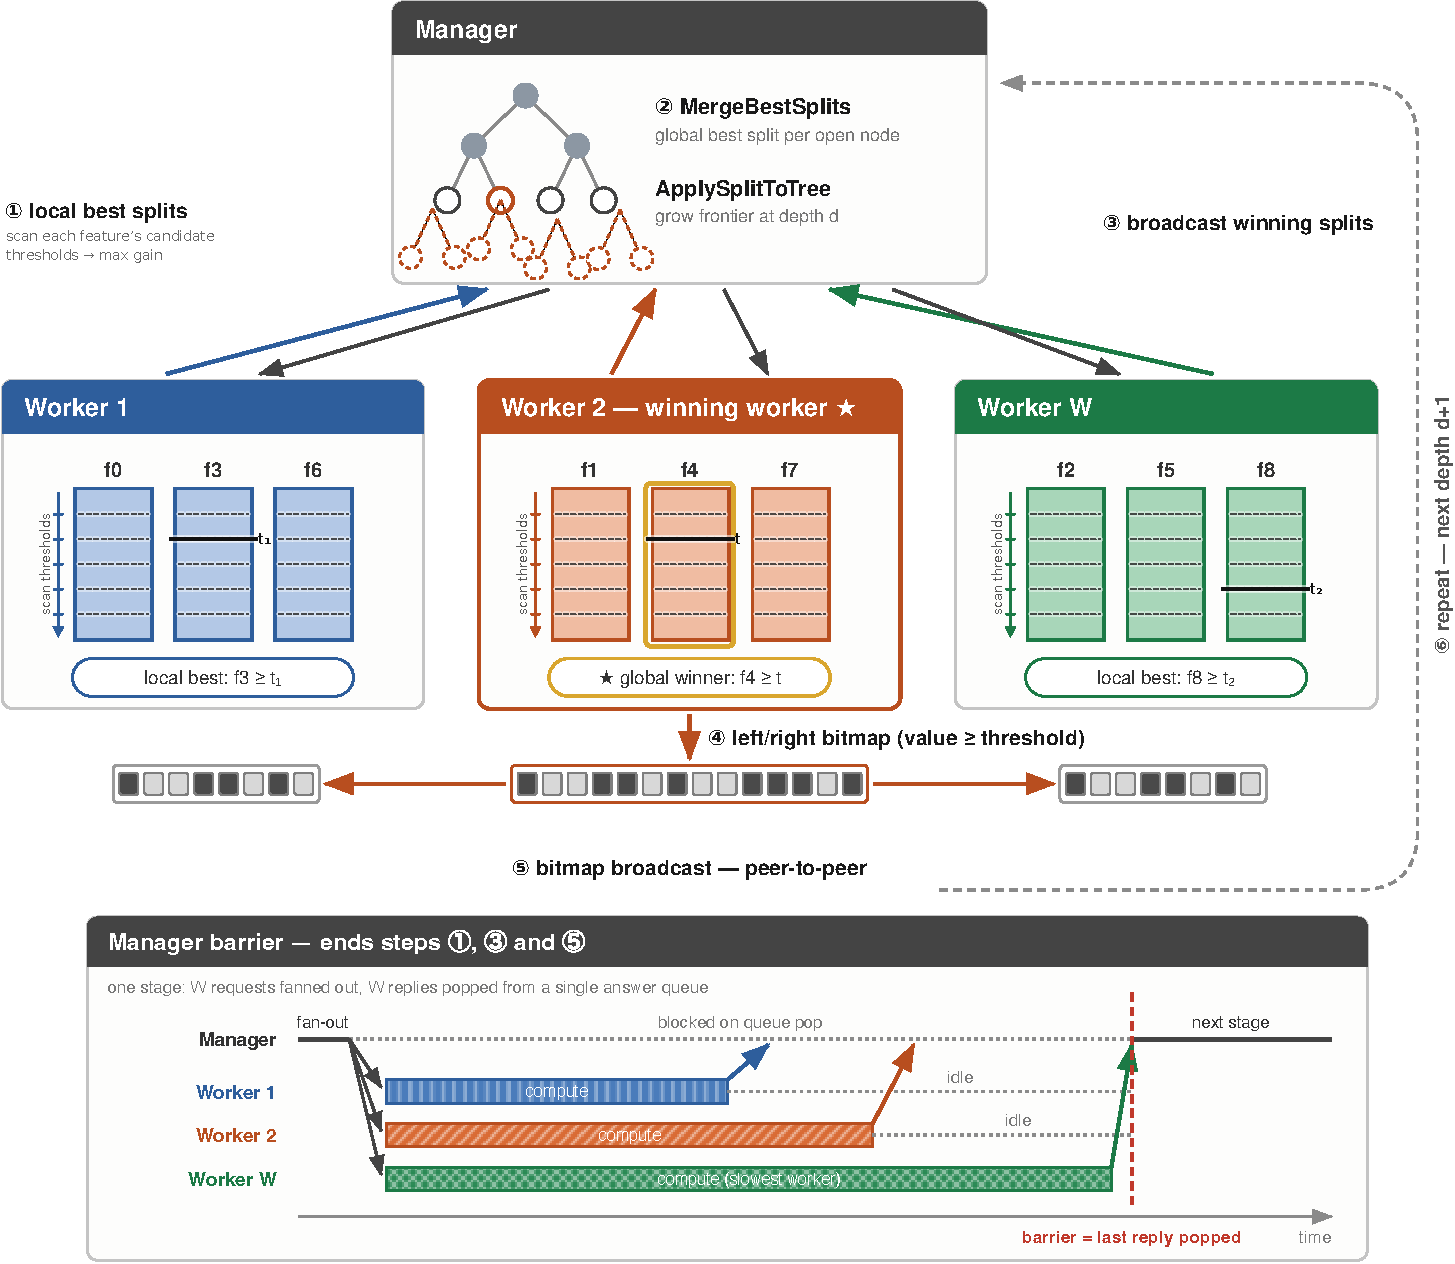
\includegraphics[width=.72\linewidth]{figures/method/distributed_gbt_training_loop_barrier.pdf}
    \caption{Distributed GBT Training Loop and manager barrier.}
    \label{fig:ydf-dist-gbt-training-loop}
\end{figure*}

\subsubsection{Load-balanced Data Sharding}

\begin{figure}[H]
    \centering
    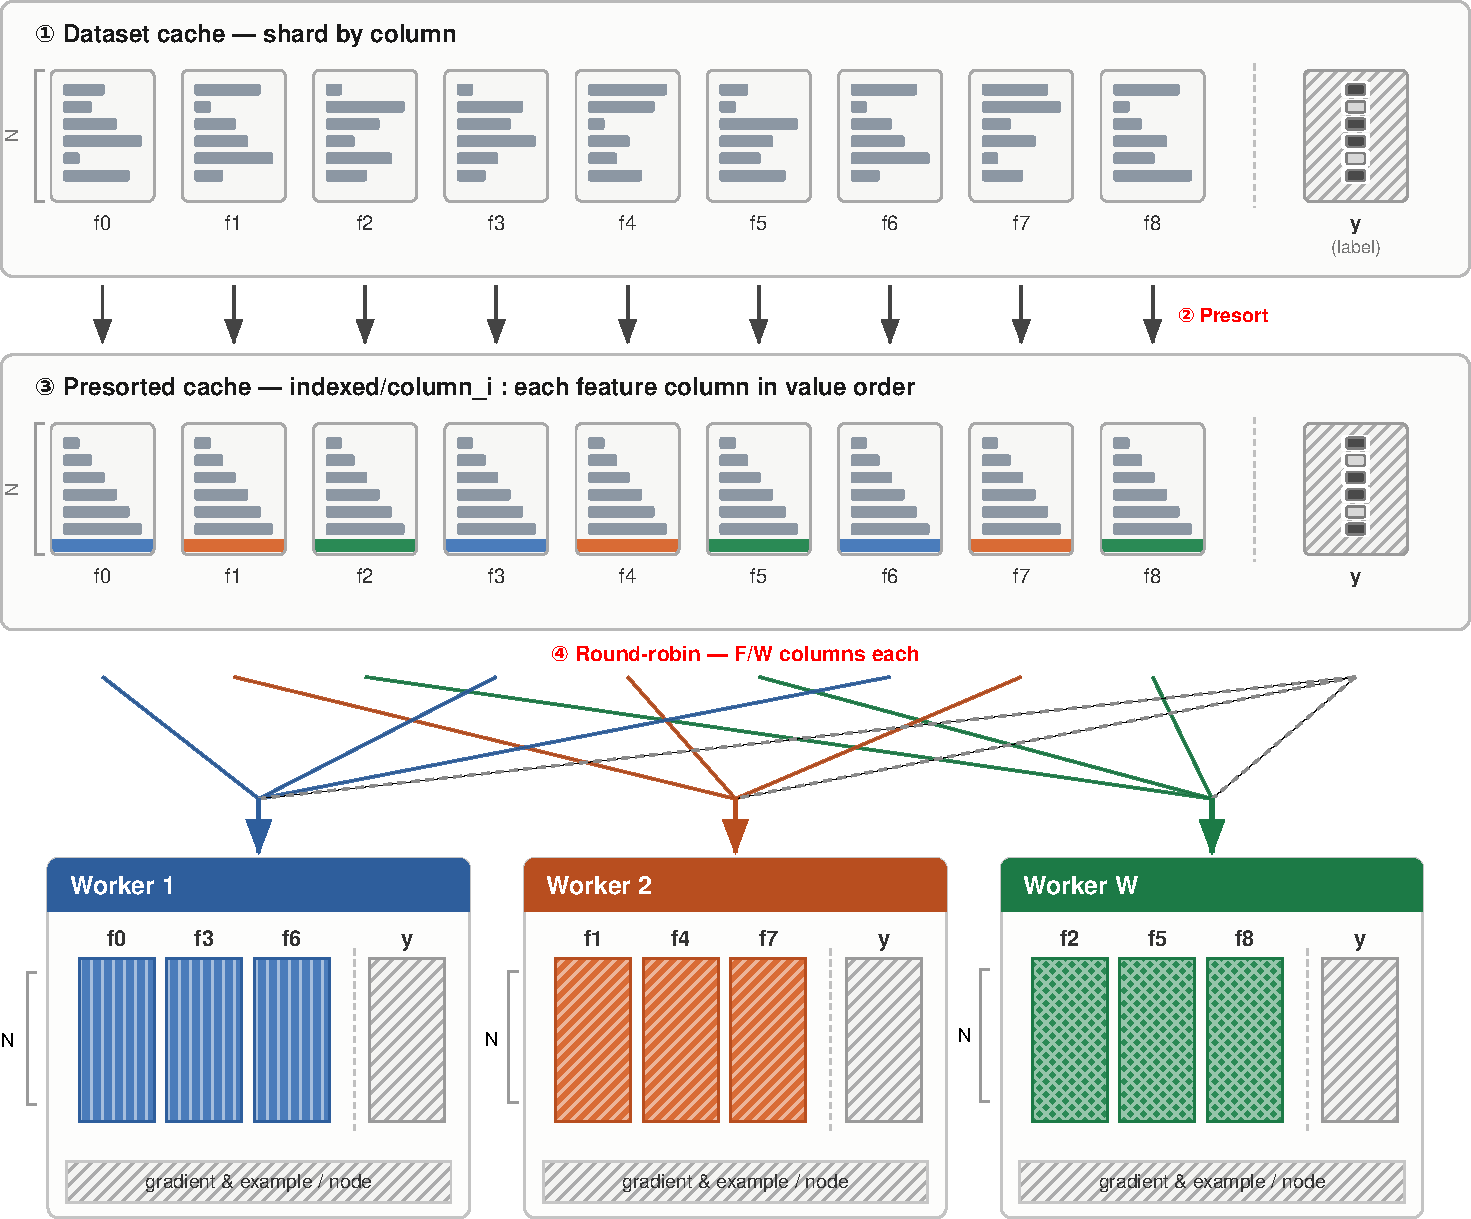
\includegraphics[width=1\linewidth]{figures/method/distributed_gbt_column_partitioning.pdf}
    \caption{Data Sharding illustration. Dataset is split by column, presorted, then round-robined in a load-balancing way.}
    \label{fig:ydf-dist-gbt-load-balancing}
\end{figure}

Feature columns are weighed by their expected compute expense : numerical features weigh $5.0$, Discretized weigh $1.0$ (\texttt{LoadBalancer::Initialize}). Numerical columns are Pre-Sorted (\texttt{dataset\_cache.cc::SortNumericalColumns}).

\begin{enumerate}
    \item Shard dataset in shared directory, by column. 
        \begin{itemize}
            \item 1 column to 1 worker. No replication.
            \item \textbf{Main issue}: how to shard these once in SPO when they're sampled per node?
        \end{itemize}
    \item Presort Columns. \textbf{Not possible in SPO}
    \item Load-balanced column round-robin to workers, by compute intensity: 5 for Numeric, 1 for Discretized. \textbf{Issue 3. No fixed columns in SPO}
    \item Train
\end{enumerate}

\subsubsection{Training}

\paragraph{for depth in tree:}

\begin{enumerate}
    \item Workers scan their column subset, computing local \texttt{BestSplit} for nodes at a depth $d$ (in \texttt{FindBestSplitsWithThreadPool}). Local maxes are sent to Manager.
    \item Manager computes global Max in \texttt{MergeBestSplits}. Update manager's tree structure \texttt{ApplySplitToTree}.
    \item Manager broadcasts global winning split - \texttt{EmitEvaluateSplits}
    \item Worker who owns Winning Column creates \textbf{bitmap} of examples to split into left-right. There is 1 winner per node at this depth
        \begin{lstlisting}
for (auto value : values) {
  const auto node_idx = example_to_node[example_idx];
  if (active_node_idx >= 0)
    active_node.writer.Write(value >= active_node.threshold);  // the bitmap
  example_idx++;
}
        \end{lstlisting}
    \item Winning workers broadcasts bitmap peer-to-peer
    \item Monitor workload for skew. Work-steal.
\end{enumerate}


\subsection{Approximate Splits}

\TODO{check if this is being used}

\textbf{Consider using approximate splits} to further improve training speed. Very often, this can speed up training by 2x-5x without negative impact on quality. Set hyperparameter\\ \textbf{force\_numerical\_discretization=True} to enable approximate splits for distributed training.

\section{Related Work}

\TODO{summarize}


\section{Method: Column Distribution Strategies on Distributed SPO-GBT}

Partitioning function should be done when loading data - where VerticalDataset is created. Still TODO: decide partitioning fn.

\subsection{All Columns on Every Worker}

\TODO{What does this experiment tell us?}

In GBT, each worker (tree) node scans all $\mathbf{F}$ columns, unlike RF and SPO-RF, which sample $\sqrt{\mathbf{F}} \sim \mathbf{F}$. \newline

\textbf{\textit{Benefit}}: Full feature range available for sampling

\textbf{\textit{Cost:}} Requires many-to-many communication at each depth, as no single node holds all features.


\subsection{V0: $\frac{F}{W}$ Worker-local projections}

% Also applicable to bivariate and other random subset-based tree kernels

% \begin{figure}
%     \centering
%     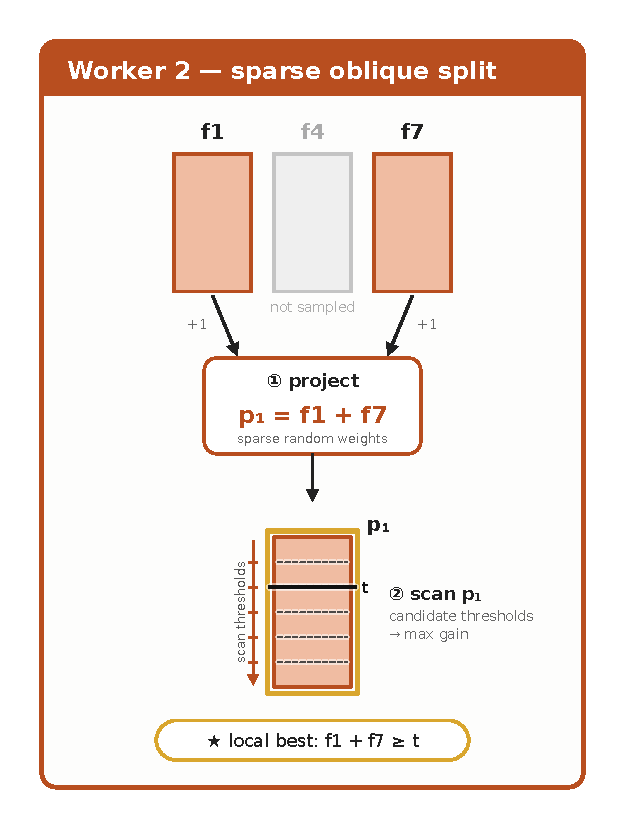
\includegraphics[width=.6\linewidth]{figures/method/in_node_spo_sampling.pdf}
%     \caption{V1 works identically to Distributed GBT, but features are sampled only within a worker.}
%     \label{fig:simple-in-worker-column-sampling}
% \end{figure}

% \begin{figure}[t]
% \begin{lstlisting}[basicstyle=\ttfamily\scriptsize]
% if (oblique) {
%   const int num_features_for_projection_count =
%       spe_config.in_worker_oblique().num_projections_from_local_features()
%           ? 0
%           : num_global_numerical_features_;
%   for (int weak_model_idx = 0; weak_model_idx < weak_models_.size();
%        weak_model_idx++) {
%     auto& weak_model = weak_models_[weak_model_idx];
%     const distributed_decision_tree::ObliqueSplitArgs args{
%         oblique_features_per_weak_models[weak_model_idx],
%         weak_model.example_to_node,
%         welcome_.dataspec(),
%         welcome_.train_config_linking(),
%         dt_config,
%         *weak_model.label_accessor,
%         weak_model.label_stats_per_node,
%         *oblique_columns_,
%         model::proto::Task::REGRESSION,
%         weak_model.label_accessor_type,
%         num_features_for_projection_count,
%         MixProjectionSeed(request.projection_seed(), WorkerIdx(),
%                           weak_model_idx)};
%     RETURN_IF_ERROR(distributed_decision_tree::FindBestObliqueSplits(
%         args, thread_pool_.get(), &splits_per_weak_models[weak_model_idx]));
%   }
% }
% \end{lstlisting}
% \caption{Worker-side call into the in-worker oblique split search (\texttt{worker.cc}, \texttt{FindSplits}).}
% \label{lst:worker_oblique_call}
% \end{figure}

Load balancing disabled for Dist. SPO-GBT


Each worker holds and samples from a small subset of columns.

\textbf{\textit{How many features should each worker hold?}}

Define $F_{\text{node}} \coloneqq \mathbf{F}$ as the number of columns stored at each worker.



\begin{description}
    \item[\textit{Benefit}:]
    \begin{itemize}
        \item No communication
    \end{itemize}
\end{description}

\begin{description}
    \item[\textit{Cost}:]
    \begin{itemize}
        \item Smaller search space than sampling $F \sim \mathbf{F}$.
        \item Each worker still needs to hold $F$ features instead of 1.
    \end{itemize}
\end{description}


\subsection{Random Column Assignment}

\subsection{$C_2$ Combinations}

\subsection{Smart Column Assignments}

Frequently-selected columns \TODO{plot this}, Correlation-based, Information per column, Vova sketching

measure accuracy of each

Figure~\ref{fig:cc18-tree1-pareto} shows which features the trees of an axis-aligned GBT split on.

\begin{figure*}[t]
\centering
\definecolor{paretoblue}{HTML}{3B6EA8}
\definecolor{paretoorange}{HTML}{F28E2B}
{\footnotesize\bfseries Tree 1}\par\nopagebreak\vspace{-0.6ex}
\begin{tikzpicture}
\begin{groupplot}[group style={group size=3 by 2, horizontal sep=1.0cm, vertical sep=1.05cm,
    xlabels at=edge bottom, ylabels at=edge left},
  width=0.333\textwidth, height=2.7cm, ymin=0, enlarge y limits={upper, value=0.08},
  ylabel={share (\%)}, ybar, /pgf/bar width=0.8,
  tick label style={font=\scriptsize}, label style={font=\scriptsize}, title style={font=\scriptsize, yshift=-1ex},
  xmin=0.4, enlarge x limits=false, scaled ticks=false]
% tree 1 row1 #1: tree-1 normalised entropy 0.902
\nextgroupplot[title={diabetes (8/8)}, xmax=8.6, xtick={1,...,8}]
\addplot[draw=none, fill={paretoblue}] table[x=rank, y=share_pct] {figures/evaluation/cc18_tree1_pareto/row11_t1.dat};
% tree 1 row1 #2: tree-1 normalised entropy 0.913
\nextgroupplot[title={breast-w (9/9)}, xmax=9.6, xtick={1,...,9}]
\addplot[draw=none, fill={paretoblue}] table[x=rank, y=share_pct] {figures/evaluation/cc18_tree1_pareto/row12_t1.dat};
% tree 1 row1 #3: tree-1 normalised entropy 0.979
\nextgroupplot[title={tic-tac-toe (9/9)}, xmax=9.6, xtick={1,...,9}]
\addplot[draw=none, fill={paretoblue}] table[x=rank, y=share_pct] {figures/evaluation/cc18_tree1_pareto/row13_t1.dat};
% tree 1 row2 #1: tree-1 normalised entropy 0.914
\nextgroupplot[title={dresses-sales (11/12)}, xmax=11.6, xtick={1,...,11}]
\addplot[draw=none, fill={paretoblue}] table[x=rank, y=share_pct] {figures/evaluation/cc18_tree1_pareto/row21_t1.dat};
% tree 1 row2 #2: tree-1 normalised entropy 0.852
\nextgroupplot[title={pc4 (30/37)}, xmax=30.6, xtick={1,30}]
\addplot[draw=none, fill={paretoblue}] table[x=rank, y=share_pct] {figures/evaluation/cc18_tree1_pareto/row22_t1.dat};
% tree 1 row2 #3: tree-1 normalised entropy 0.596
\nextgroupplot[title={Bioresponse (120/1776)}, xmax=120.6, xtick={1,120}]
\addplot[draw=none, fill={paretoblue}] table[x=rank, y=share_pct] {figures/evaluation/cc18_tree1_pareto/row23_t1.dat};
\end{groupplot}
\end{tikzpicture}
\par\vspace{0.2ex}
{\footnotesize\bfseries Tree 100}\par\nopagebreak\vspace{-0.6ex}
\begin{tikzpicture}
\begin{groupplot}[group style={group size=3 by 2, horizontal sep=1.0cm, vertical sep=1.05cm,
    xlabels at=edge bottom, ylabels at=edge left},
  width=0.333\textwidth, height=2.7cm, ymin=0, enlarge y limits={upper, value=0.08},
  ylabel={share (\%)}, ybar, /pgf/bar width=0.8,
  tick label style={font=\scriptsize}, label style={font=\scriptsize}, title style={font=\scriptsize, yshift=-1ex},
  xmin=0.4, enlarge x limits=false, scaled ticks=false]
% tree 100 row1 #1: tree-1 normalised entropy 0.902
\nextgroupplot[title={diabetes (8/8)}, xmax=8.6, xtick={1,...,8}]
\addplot[draw=none, fill={paretoblue}] table[x=rank, y=share_pct] {figures/evaluation/cc18_tree1_pareto/row11_t100.dat};
% tree 100 row1 #2: tree-1 normalised entropy 0.913
\nextgroupplot[title={breast-w (9/9)}, xmax=9.6, xtick={1,...,9}]
\addplot[draw=none, fill={paretoblue}] table[x=rank, y=share_pct] {figures/evaluation/cc18_tree1_pareto/row12_t100.dat};
% tree 100 row1 #3: tree-1 normalised entropy 0.979
\nextgroupplot[title={tic-tac-toe (9/9)}, xmax=9.6, xtick={1,...,9}]
\addplot[draw=none, fill={paretoblue}] table[x=rank, y=share_pct] {figures/evaluation/cc18_tree1_pareto/row13_t100.dat};
% tree 100 row2 #1: tree-1 normalised entropy 0.914
\nextgroupplot[title={dresses-sales (12/12)}, xmax=12.6, xtick={1,...,12}]
\addplot[draw=none, fill={paretoblue}] table[x=rank, y=share_pct] {figures/evaluation/cc18_tree1_pareto/row21_t100.dat};
% tree 100 row2 #2: tree-1 normalised entropy 0.852
\nextgroupplot[title={pc4 (35/37)}, xmax=35.6, xtick={1,35}]
\addplot[draw=none, fill={paretoblue}] table[x=rank, y=share_pct] {figures/evaluation/cc18_tree1_pareto/row22_t100.dat};
% tree 100 row2 #3: tree-1 normalised entropy 0.596
\nextgroupplot[title={Bioresponse (120/1776)}, xmax=120.6, xtick={1,120}]
\addplot[draw=none, fill={paretoblue}] table[x=rank, y=share_pct] {figures/evaluation/cc18_tree1_pareto/row23_t100.dat};
\end{groupplot}
\end{tikzpicture}
\par\vspace{0.2ex}
{\footnotesize\bfseries Tree 200}\par\nopagebreak\vspace{-0.6ex}
\begin{tikzpicture}
\begin{groupplot}[group style={group size=3 by 2, horizontal sep=1.0cm, vertical sep=1.05cm,
    xlabels at=edge bottom, ylabels at=edge left},
  width=0.333\textwidth, height=2.7cm, ymin=0, enlarge y limits={upper, value=0.08},
  ylabel={share (\%)}, ybar, /pgf/bar width=0.8,
  tick label style={font=\scriptsize}, label style={font=\scriptsize}, title style={font=\scriptsize, yshift=-1ex},
  xmin=0.4, enlarge x limits=false, scaled ticks=false]
% tree 200 row1 #1: tree-1 normalised entropy 0.902
\nextgroupplot[title={diabetes (8/8)}, xmax=8.6, xtick={1,...,8}]
\addplot[draw=none, fill={paretoblue}] table[x=rank, y=share_pct] {figures/evaluation/cc18_tree1_pareto/row11_t200.dat};
% tree 200 row1 #2: tree-1 normalised entropy 0.913
\nextgroupplot[title={breast-w (9/9)}, xmax=9.6, xtick={1,...,9}]
\addplot[draw=none, fill={paretoblue}] table[x=rank, y=share_pct] {figures/evaluation/cc18_tree1_pareto/row12_t200.dat};
% tree 200 row1 #3: tree-1 normalised entropy 0.979
\nextgroupplot[title={tic-tac-toe (9/9)}, xmax=9.6, xtick={1,...,9}]
\addplot[draw=none, fill={paretoblue}] table[x=rank, y=share_pct] {figures/evaluation/cc18_tree1_pareto/row13_t200.dat};
% tree 200 row2 #1: tree-1 normalised entropy 0.914
\nextgroupplot[title={dresses-sales (11/12)}, xmax=11.6, xtick={1,...,11}]
\addplot[draw=none, fill={paretoblue}] table[x=rank, y=share_pct] {figures/evaluation/cc18_tree1_pareto/row21_t200.dat};
% tree 200 row2 #2: tree-1 normalised entropy 0.852
\nextgroupplot[title={pc4 (35/37)}, xmax=35.6, xtick={1,35}]
\addplot[draw=none, fill={paretoblue}] table[x=rank, y=share_pct] {figures/evaluation/cc18_tree1_pareto/row22_t200.dat};
% tree 200 row2 #3: tree-1 normalised entropy 0.596
\nextgroupplot[title={Bioresponse (132/1776)}, xmax=132.6, xtick={1,132}]
\addplot[draw=none, fill={paretoblue}] table[x=rank, y=share_pct] {figures/evaluation/cc18_tree1_pareto/row23_t200.dat};
\end{groupplot}
\end{tikzpicture}
\par\vspace{0.2ex}
{\footnotesize\bfseries Tree 300}\par\nopagebreak\vspace{-0.6ex}
\begin{tikzpicture}
\begin{groupplot}[group style={group size=3 by 2, horizontal sep=1.0cm, vertical sep=1.05cm,
    xlabels at=edge bottom, ylabels at=edge left},
  width=0.333\textwidth, height=2.7cm, ymin=0, enlarge y limits={upper, value=0.08},
  xlabel={feature rank}, ylabel={share (\%)}, ybar, /pgf/bar width=0.8,
  tick label style={font=\scriptsize}, label style={font=\scriptsize}, title style={font=\scriptsize, yshift=-1ex},
  xmin=0.4, enlarge x limits=false, scaled ticks=false]
% tree 300 row1 #1: tree-1 normalised entropy 0.902
\nextgroupplot[title={diabetes (8/8)}, xmax=8.6, xtick={1,...,8}]
\addplot[draw=none, fill={paretoblue}] table[x=rank, y=share_pct] {figures/evaluation/cc18_tree1_pareto/row11_t300.dat};
% tree 300 row1 #2: tree-1 normalised entropy 0.913
\nextgroupplot[title={breast-w (9/9)}, xmax=9.6, xtick={1,...,9}]
\addplot[draw=none, fill={paretoblue}] table[x=rank, y=share_pct] {figures/evaluation/cc18_tree1_pareto/row12_t300.dat};
% tree 300 row1 #3: tree-1 normalised entropy 0.979
\nextgroupplot[title={tic-tac-toe (9/9)}, xmax=9.6, xtick={1,...,9}]
\addplot[draw=none, fill={paretoblue}] table[x=rank, y=share_pct] {figures/evaluation/cc18_tree1_pareto/row13_t300.dat};
% tree 300 row2 #1: tree-1 normalised entropy 0.914
\nextgroupplot[title={dresses-sales (12/12)}, xmax=12.6, xtick={1,...,12}]
\addplot[draw=none, fill={paretoblue}] table[x=rank, y=share_pct] {figures/evaluation/cc18_tree1_pareto/row21_t300.dat};
% tree 300 row2 #2: tree-1 normalised entropy 0.852
\nextgroupplot[title={pc4 (35/37)}, xmax=35.6, xtick={1,35}]
\addplot[draw=none, fill={paretoblue}] table[x=rank, y=share_pct] {figures/evaluation/cc18_tree1_pareto/row22_t300.dat};
% tree 300 row2 #3: tree-1 normalised entropy 0.596
\nextgroupplot[title={Bioresponse (107/1776)}, xmax=107.6, xtick={1,107}]
\addplot[draw=none, fill={paretoblue}] table[x=rank, y=share_pct] {figures/evaluation/cc18_tree1_pareto/row23_t300.dat};
\end{groupplot}
\end{tikzpicture}

\caption{Features split on by the first tree of a AA-GBT. Top: most Pareto-like. Bottom: least-pareto like. \TODO{does this remain the same for latter GBTs? Tradeoff of Extra memory vs. Accuracy}}
\Description{Six bar charts of per-feature split share in the first GBT tree, sorted descending, for three concentrated and three flat datasets.}
\label{fig:cc18-tree1-pareto}
\par\smallskip\raggedright\footnotesize pooled over the 10 cross-validation models of a dataset
\end{figure*}

\begin{figure*}[t]
\centering
\definecolor{paretoblue}{HTML}{3B6EA8}
\definecolor{paretoorange}{HTML}{F28E2B}
{\footnotesize\bfseries Tree 1}\par\nopagebreak\vspace{-0.6ex}
\begin{tikzpicture}
\begin{groupplot}[group style={group size=3 by 2, horizontal sep=1.0cm, vertical sep=1.05cm,
    xlabels at=edge bottom, ylabels at=edge left},
  width=0.333\textwidth, height=2.7cm, ymin=0,
  ylabel={share (\%)},
  tick label style={font=\scriptsize}, label style={font=\scriptsize}, title style={font=\scriptsize, yshift=-1ex},
  enlarge x limits=false, scaled ticks=false]
% tree 1 row1 #1: tree-1 normalised entropy 0.902
\nextgroupplot[title={diabetes (8/8)}, xmin=0.5, xmax=8.5, xtick={1,...,8}, ymax=27.885]
\addplot[ybar, draw=none, fill=paretoblue, /pgf/bar width=0.8] table[x=x, y=share_pct] {figures/evaluation/cc18_tree_feature_hist/row11_t1.dat};
% tree 1 row1 #2: tree-1 normalised entropy 0.913
\nextgroupplot[title={breast-w (9/9)}, xmin=0.5, xmax=9.5, xtick={1,...,9}, ymax=23.538]
\addplot[ybar, draw=none, fill=paretoblue, /pgf/bar width=0.8] table[x=x, y=share_pct] {figures/evaluation/cc18_tree_feature_hist/row12_t1.dat};
% tree 1 row1 #3: tree-1 normalised entropy 0.979
\nextgroupplot[title={tic-tac-toe (9/9)}, xmin=0.5, xmax=9.5, xtick={1,...,9}, ymax=17.405]
\addplot[ybar, draw=none, fill=paretoblue, /pgf/bar width=0.8] table[x=x, y=share_pct] {figures/evaluation/cc18_tree_feature_hist/row13_t1.dat};
% tree 1 row2 #1: tree-1 normalised entropy 0.914
\nextgroupplot[title={dresses-sales (11/12)}, xmin=0.5, xmax=12.5, xtick={1,...,12}, ymax=18.655]
\addplot[ybar, draw=none, fill=paretoblue, /pgf/bar width=0.8] table[x=x, y=share_pct] {figures/evaluation/cc18_tree_feature_hist/row21_t1.dat};
% tree 1 row2 #2: tree-1 normalised entropy 0.852
\nextgroupplot[title={pc4 (30/37)}, xmin=0.5, xmax=37.5, xtick={1,37}, ymax=17.514]
\addplot[ybar, draw=none, fill=paretoblue, /pgf/bar width=0.8] table[x=x, y=share_pct] {figures/evaluation/cc18_tree_feature_hist/row22_t1.dat};
% tree 1 row2 #3: tree-1 normalised entropy 0.596
\nextgroupplot[title={Bioresponse (120/1776)}, xmin=0.5, xmax=1776.5, xtick={1,1776}, ymax=4.612]
\addplot[ycomb, paretoblue, line width=0.35pt, mark=none] table[x=x, y=share_pct] {figures/evaluation/cc18_tree_feature_hist/row23_t1.dat};
\end{groupplot}
\end{tikzpicture}
\par\vspace{0.2ex}
{\footnotesize\bfseries Tree 100}\par\nopagebreak\vspace{-0.6ex}
\begin{tikzpicture}
\begin{groupplot}[group style={group size=3 by 2, horizontal sep=1.0cm, vertical sep=1.05cm,
    xlabels at=edge bottom, ylabels at=edge left},
  width=0.333\textwidth, height=2.7cm, ymin=0,
  ylabel={share (\%)},
  tick label style={font=\scriptsize}, label style={font=\scriptsize}, title style={font=\scriptsize, yshift=-1ex},
  enlarge x limits=false, scaled ticks=false]
% tree 100 row1 #1: tree-1 normalised entropy 0.902
\nextgroupplot[title={diabetes (8/8)}, xmin=0.5, xmax=8.5, xtick={1,...,8}, ymax=27.885]
\addplot[ybar, draw=none, fill=paretoblue, /pgf/bar width=0.8] table[x=x, y=share_pct] {figures/evaluation/cc18_tree_feature_hist/row11_t100.dat};
% tree 100 row1 #2: tree-1 normalised entropy 0.913
\nextgroupplot[title={breast-w (9/9)}, xmin=0.5, xmax=9.5, xtick={1,...,9}, ymax=23.538]
\addplot[ybar, draw=none, fill=paretoblue, /pgf/bar width=0.8] table[x=x, y=share_pct] {figures/evaluation/cc18_tree_feature_hist/row12_t100.dat};
% tree 100 row1 #3: tree-1 normalised entropy 0.979
\nextgroupplot[title={tic-tac-toe (9/9)}, xmin=0.5, xmax=9.5, xtick={1,...,9}, ymax=17.405]
\addplot[ybar, draw=none, fill=paretoblue, /pgf/bar width=0.8] table[x=x, y=share_pct] {figures/evaluation/cc18_tree_feature_hist/row13_t100.dat};
% tree 100 row2 #1: tree-1 normalised entropy 0.914
\nextgroupplot[title={dresses-sales (12/12)}, xmin=0.5, xmax=12.5, xtick={1,...,12}, ymax=18.655]
\addplot[ybar, draw=none, fill=paretoblue, /pgf/bar width=0.8] table[x=x, y=share_pct] {figures/evaluation/cc18_tree_feature_hist/row21_t100.dat};
% tree 100 row2 #2: tree-1 normalised entropy 0.852
\nextgroupplot[title={pc4 (35/37)}, xmin=0.5, xmax=37.5, xtick={1,37}, ymax=17.514]
\addplot[ybar, draw=none, fill=paretoblue, /pgf/bar width=0.8] table[x=x, y=share_pct] {figures/evaluation/cc18_tree_feature_hist/row22_t100.dat};
% tree 100 row2 #3: tree-1 normalised entropy 0.596
\nextgroupplot[title={Bioresponse (120/1776)}, xmin=0.5, xmax=1776.5, xtick={1,1776}, ymax=4.612]
\addplot[ycomb, paretoblue, line width=0.35pt, mark=none] table[x=x, y=share_pct] {figures/evaluation/cc18_tree_feature_hist/row23_t100.dat};
\end{groupplot}
\end{tikzpicture}
\par\vspace{0.2ex}
{\footnotesize\bfseries Tree 200}\par\nopagebreak\vspace{-0.6ex}
\begin{tikzpicture}
\begin{groupplot}[group style={group size=3 by 2, horizontal sep=1.0cm, vertical sep=1.05cm,
    xlabels at=edge bottom, ylabels at=edge left},
  width=0.333\textwidth, height=2.7cm, ymin=0,
  ylabel={share (\%)},
  tick label style={font=\scriptsize}, label style={font=\scriptsize}, title style={font=\scriptsize, yshift=-1ex},
  enlarge x limits=false, scaled ticks=false]
% tree 200 row1 #1: tree-1 normalised entropy 0.902
\nextgroupplot[title={diabetes (8/8)}, xmin=0.5, xmax=8.5, xtick={1,...,8}, ymax=27.885]
\addplot[ybar, draw=none, fill=paretoblue, /pgf/bar width=0.8] table[x=x, y=share_pct] {figures/evaluation/cc18_tree_feature_hist/row11_t200.dat};
% tree 200 row1 #2: tree-1 normalised entropy 0.913
\nextgroupplot[title={breast-w (9/9)}, xmin=0.5, xmax=9.5, xtick={1,...,9}, ymax=23.538]
\addplot[ybar, draw=none, fill=paretoblue, /pgf/bar width=0.8] table[x=x, y=share_pct] {figures/evaluation/cc18_tree_feature_hist/row12_t200.dat};
% tree 200 row1 #3: tree-1 normalised entropy 0.979
\nextgroupplot[title={tic-tac-toe (9/9)}, xmin=0.5, xmax=9.5, xtick={1,...,9}, ymax=17.405]
\addplot[ybar, draw=none, fill=paretoblue, /pgf/bar width=0.8] table[x=x, y=share_pct] {figures/evaluation/cc18_tree_feature_hist/row13_t200.dat};
% tree 200 row2 #1: tree-1 normalised entropy 0.914
\nextgroupplot[title={dresses-sales (11/12)}, xmin=0.5, xmax=12.5, xtick={1,...,12}, ymax=18.655]
\addplot[ybar, draw=none, fill=paretoblue, /pgf/bar width=0.8] table[x=x, y=share_pct] {figures/evaluation/cc18_tree_feature_hist/row21_t200.dat};
% tree 200 row2 #2: tree-1 normalised entropy 0.852
\nextgroupplot[title={pc4 (35/37)}, xmin=0.5, xmax=37.5, xtick={1,37}, ymax=17.514]
\addplot[ybar, draw=none, fill=paretoblue, /pgf/bar width=0.8] table[x=x, y=share_pct] {figures/evaluation/cc18_tree_feature_hist/row22_t200.dat};
% tree 200 row2 #3: tree-1 normalised entropy 0.596
\nextgroupplot[title={Bioresponse (132/1776)}, xmin=0.5, xmax=1776.5, xtick={1,1776}, ymax=4.612]
\addplot[ycomb, paretoblue, line width=0.35pt, mark=none] table[x=x, y=share_pct] {figures/evaluation/cc18_tree_feature_hist/row23_t200.dat};
\end{groupplot}
\end{tikzpicture}
\par\vspace{0.2ex}
{\footnotesize\bfseries Tree 300}\par\nopagebreak\vspace{-0.6ex}
\begin{tikzpicture}
\begin{groupplot}[group style={group size=3 by 2, horizontal sep=1.0cm, vertical sep=1.05cm,
    xlabels at=edge bottom, ylabels at=edge left},
  width=0.333\textwidth, height=2.7cm, ymin=0,
  xlabel={feature index (header order)}, ylabel={share (\%)},
  tick label style={font=\scriptsize}, label style={font=\scriptsize}, title style={font=\scriptsize, yshift=-1ex},
  enlarge x limits=false, scaled ticks=false]
% tree 300 row1 #1: tree-1 normalised entropy 0.902
\nextgroupplot[title={diabetes (8/8)}, xmin=0.5, xmax=8.5, xtick={1,...,8}, ymax=27.885]
\addplot[ybar, draw=none, fill=paretoblue, /pgf/bar width=0.8] table[x=x, y=share_pct] {figures/evaluation/cc18_tree_feature_hist/row11_t300.dat};
% tree 300 row1 #2: tree-1 normalised entropy 0.913
\nextgroupplot[title={breast-w (9/9)}, xmin=0.5, xmax=9.5, xtick={1,...,9}, ymax=23.538]
\addplot[ybar, draw=none, fill=paretoblue, /pgf/bar width=0.8] table[x=x, y=share_pct] {figures/evaluation/cc18_tree_feature_hist/row12_t300.dat};
% tree 300 row1 #3: tree-1 normalised entropy 0.979
\nextgroupplot[title={tic-tac-toe (9/9)}, xmin=0.5, xmax=9.5, xtick={1,...,9}, ymax=17.405]
\addplot[ybar, draw=none, fill=paretoblue, /pgf/bar width=0.8] table[x=x, y=share_pct] {figures/evaluation/cc18_tree_feature_hist/row13_t300.dat};
% tree 300 row2 #1: tree-1 normalised entropy 0.914
\nextgroupplot[title={dresses-sales (12/12)}, xmin=0.5, xmax=12.5, xtick={1,...,12}, ymax=18.655]
\addplot[ybar, draw=none, fill=paretoblue, /pgf/bar width=0.8] table[x=x, y=share_pct] {figures/evaluation/cc18_tree_feature_hist/row21_t300.dat};
% tree 300 row2 #2: tree-1 normalised entropy 0.852
\nextgroupplot[title={pc4 (35/37)}, xmin=0.5, xmax=37.5, xtick={1,37}, ymax=17.514]
\addplot[ybar, draw=none, fill=paretoblue, /pgf/bar width=0.8] table[x=x, y=share_pct] {figures/evaluation/cc18_tree_feature_hist/row22_t300.dat};
% tree 300 row2 #3: tree-1 normalised entropy 0.596
\nextgroupplot[title={Bioresponse (107/1776)}, xmin=0.5, xmax=1776.5, xtick={1,1776}, ymax=4.612]
\addplot[ycomb, paretoblue, line width=0.35pt, mark=none] table[x=x, y=share_pct] {figures/evaluation/cc18_tree_feature_hist/row23_t300.dat};
\end{groupplot}
\end{tikzpicture}

\caption{Same trees as Figure~\ref{fig:cc18-tree1-pareto} on a fixed x-axis: the dataset's features in header order (unused features at 0), so the feature set is identical across the tree blocks and only the distribution of splits moves. Same y range per dataset.}
\Description{Bar charts of per-feature split share against feature index for the same six datasets and trees 1, 100, 200 and 300.}
\label{fig:cc18-tree-feature-hist}
\par\smallskip\raggedright\footnotesize pooled over the 10 cross-validation models of a dataset
\end{figure*}

\section{Evaluation}

\begin{table*}[t]
\centering\footnotesize\setlength{\tabcolsep}{4pt}
\caption{Distributed tree-training time (s) on Vertex AI \texttt{n2-highmem-4} (left) and \texttt{n2-highmem-16} (right), $P{=}F$ projections}
\label{tab:vertex-hm4-pf-runtime}
% auto-generated by benchmarks/src/distributed_spo_gbt/make_pf_grid_table.py -- regenerate, do not hand-edit
% cells: runtime/distributed_spo_gbt/barriers/vertex/pfhm4_20261025*, n2-highmem-4 | pfgrid20261025*, n2-highmem-16, 10 trees
\begin{tabular}{ll|rrrrr|r||rrr|r}
\toprule
 & & \multicolumn{6}{c||}{\textbf{\texttt{n2-highmem-4}}} & \multicolumn{4}{c}{\textbf{\texttt{n2-highmem-16}}} \\
Dataset & Arm & $W=1$ & $W=2$ & $W=4$ & $W=8$ & $W=16$ & Acc. & $W=1$ & $W=2$ & $W=4$ & Acc. \\
\midrule
Epsilon & AA & 716 & 366 & 193 & 98 & 50 & 0.719 & 133 & 68 & 35 & 0.719 \\
 & SPO in-node & 728 & 375 & 184 & 97 & 49 & 0.726--0.732 & 134 & 67 & 35 & 0.726--0.732 \\
\midrule
HIGGS & AA & 472 & 250 & 147 & 84 & 80 & 0.688 & 97 & 72 & 72 & 0.688 \\
 & SPO in-node & 532 & 292 & 150 & 79 & 42 & 0.683--0.692 & 115 & 65 & 43 & 0.689--0.692 \\
\midrule
SUSY & AA & 231 & 132 & 76 & 44 & 36 & 0.787 & 54 & 30 & 30 & 0.787 \\
 & SPO in-node & 157 & 86 & 40 & 24 & 18 & 0.785--0.789 & 37 & 23 & 15 & 0.786--0.789 \\
\midrule
YouTube-8M & AA & OOM & 6693 & 3270 & 1617 & 844 & 0.900 & 1599 & 892 & 463 & 0.900 \\
 & SPO in-node & OOM & OOM & 2135 & 1109 & 563 & 0.899 & 1326 & 670 & 375 & 0.898 \\
\bottomrule
\end{tabular}

\par\smallskip\raggedright\footnotesize In-node parallel + VQSort. $\lfloor F/W\rfloor$ per worker, so SUSY and HIGGS get 16 at $W{=}16$). 10 trees. setup excluded, checkpointing included.
\end{table*}

\begin{figure*}[t]
\centering
\begin{minipage}[b]{0.48\textwidth}
\centering
% auto-generated by benchmarks/src/distributed_spo_gbt/make_barrier_figs.py -- regenerate, do not hand-edit

\begin{tikzpicture}
\begin{axis}[width=\linewidth, height=5.2cm, ybar stacked, bar width=0.9cm, symbolic x coords={AA,SPO}, xtick=data,
  xticklabels={AA-GBT,SPO-GBT}, enlarge x limits=0.5, ymin=0, ymax=1158, ylabel={Time summed over 10 trees (s)},
  tick label style={font=\footnotesize}, label style={font=\footnotesize}, tick style={draw=none},
  legend style={font=\scriptsize, at={(0.5,-0.14)}, anchor=north, draw=none, legend columns=2, /tikz/every even column/.append style={column sep=0.6em}},
  legend cell align=left, clip=false]
\addplot[draw=none, fill={rgb,255:red,31;green,56;blue,100}] table[x=arm, y=findsplits] {figures/evaluation/grcp_n2/yt8m_barriers/totals.dat};
\addlegendentry{FindSplits compute}
\addplot[draw=none, fill={rgb,255:red,0;green,229;blue,255}] table[x=arm, y=evalsplits] {figures/evaluation/grcp_n2/yt8m_barriers/totals.dat};
\addlegendentry{EvaluateSplits compute}
\addplot[draw=none, fill={rgb,255:red,57;green,255;blue,20}] table[x=arm, y=sharesplits] {figures/evaluation/grcp_n2/yt8m_barriers/totals.dat};
\addlegendentry{ShareSplits (worker--worker comm.)}
\addplot[draw=none, fill={rgb,255:red,255;green,230;blue,0}] table[x=arm, y=startend] {figures/evaluation/grcp_n2/yt8m_barriers/totals.dat};
\addlegendentry{Tree start/end}
\addplot[draw=none, fill={rgb,255:red,255;green,0;blue,255}] table[x=arm, y=checkpoint] {figures/evaluation/grcp_n2/yt8m_barriers/totals.dat};
\addlegendentry{Checkpoints}
\addplot[draw=none, fill={rgb,255:red,255;green,95;blue,31}] table[x=arm, y=mgrcomm] {figures/evaluation/grcp_n2/yt8m_barriers/totals.dat};
\addlegendentry{Manager--worker comm.}
\node[anchor=south, font=\scriptsize, align=center, inner sep=1pt] at (axis cs:AA,827.18) {total 827.2\,s\\non-FindSplits 6.40\,s\\mgr--worker comm.\ 0.33\,s};
\node[anchor=south, font=\scriptsize, align=center, inner sep=1pt] at (axis cs:SPO,559.12) {total 559.1\,s\\non-FindSplits 5.32\,s\\mgr--worker comm.\ 0.33\,s};
\end{axis}
\end{tikzpicture}

\par\footnotesize (a) Time per barrier component, summed over the run
\end{minipage}
\hfill
\begin{minipage}[b]{0.48\textwidth}
\centering
% auto-generated by benchmarks/src/distributed_spo_gbt/make_barrier_figs.py -- regenerate, do not hand-edit

\begin{tikzpicture}
\begin{axis}[width=\linewidth, height=6.3cm, xmin=-0.5, xmax=4.5, xtick={0,...,4}, ymin=0, ymax=22,
  xlabel={Tree level}, ylabel={FindSplits time per call (s)},
  tick label style={font=\footnotesize}, label style={font=\footnotesize}, tick style={draw=none},
  legend style={font=\scriptsize, at={(0.02,0.98)}, anchor=north west, draw=none}, legend cell align=left]
\addplot[color={rgb,255:red,216;green,90;blue,48}, only marks, mark=diamond*, mark size=1.8pt, mark options={fill=white, draw=black, line width=0.4pt}, legend image code/.code={\draw[line width=4pt, color={rgb,255:red,216;green,90;blue,48}] (0.15cm,-0.13cm) -- (0.15cm,0.13cm); \draw plot[only marks, mark=diamond*, mark size=1.8pt, mark options={fill=white, draw=black, line width=0.4pt}] coordinates {(0.15cm,0cm)};},
  error bars/.cd, y dir=both, y explicit, error mark=none, error bar style={line width=4pt, color={rgb,255:red,216;green,90;blue,48}}]
  table[x expr=\thisrow{layer}-0.18, y=med_s, y error plus expr=\thisrow{max_s}-\thisrow{med_s}, y error minus expr=\thisrow{med_s}-\thisrow{min_s}] {figures/evaluation/grcp_n2/yt8m_barriers/findsplits_aa.dat};
\addlegendentry{AA-GBT}
\addplot[draw=none, forget plot, nodes near coords={\pgfmathprintnumber[fixed, precision=1]{\pgfplotspointmeta}}, nodes near coords style={font=\tiny, anchor=south, inner sep=1.5pt}, point meta=explicit]
  table[x expr=\thisrow{layer}-0.18, y=max_s, meta=idle_pct] {figures/evaluation/grcp_n2/yt8m_barriers/findsplits_aa.dat};
\addplot[color={rgb,255:red,55;green,138;blue,221}, only marks, mark=*, mark size=1.8pt, mark options={fill=white, draw=black, line width=0.4pt}, legend image code/.code={\draw[line width=4pt, color={rgb,255:red,55;green,138;blue,221}] (0.15cm,-0.13cm) -- (0.15cm,0.13cm); \draw plot[only marks, mark=*, mark size=1.8pt, mark options={fill=white, draw=black, line width=0.4pt}] coordinates {(0.15cm,0cm)};},
  error bars/.cd, y dir=both, y explicit, error mark=none, error bar style={line width=4pt, color={rgb,255:red,55;green,138;blue,221}}]
  table[x expr=\thisrow{layer}+0.18, y=med_s, y error plus expr=\thisrow{max_s}-\thisrow{med_s}, y error minus expr=\thisrow{med_s}-\thisrow{min_s}] {figures/evaluation/grcp_n2/yt8m_barriers/findsplits_spo.dat};
\addlegendentry{SPO-GBT}
\addplot[draw=none, forget plot, nodes near coords={\pgfmathprintnumber[fixed, precision=1]{\pgfplotspointmeta}}, nodes near coords style={font=\tiny, anchor=south, inner sep=1.5pt}, point meta=explicit]
  table[x expr=\thisrow{layer}+0.18, y=max_s, meta=idle_pct] {figures/evaluation/grcp_n2/yt8m_barriers/findsplits_spo.dat};
\end{axis}
\end{tikzpicture}

\par\footnotesize (b) FindSplits per tree level (labels: idle \% of worker time)
\end{minipage}
\caption{Barrier timing of distributed AA-GBT and SPO-GBT on YouTube-8M with $W{=}16$ workers on Vertex AI \texttt{n2-highmem-4} (10 trees, depth 6, $P{=}F$). (a) Stacked bars sum the slowest worker's time per stage, plus checkpoints and manager--worker communication. (b) Bars span the per-call mean of the fastest to the slowest worker's FindSplits time, markers are the median worker, and labels give the idle share of worker time.}
\Description{Two panels. Left: stacked bars of total time for AA-GBT and SPO-GBT, almost entirely FindSplits compute, annotated with the small non-FindSplits and communication totals. Right: per tree level, min-to-max range bars of FindSplits time for AA-GBT and SPO-GBT with median markers and idle percentages.}
\label{fig:yt8m-barriers}
\end{figure*}

If a dataset has no explicit test set, the last 10\% of the dataset is used as test.

\subsection{In-worker Projection Sampling}

\subsubsection{Vertex AI Results on N2-highmem}

\begin{table*}[t]
\centering
\scriptsize
\setlength{\tabcolsep}{2pt}
\caption{Mean \& std. test ROC AUC of single-machine and distributed GBT with $W$ workers, for SPO and AA over 5 CV folds. Single chronological holdouts have no std. Single-machine SPO-GBT samples $F$ projections per node, distributed SPO-GBT workers sample $F/W$ projections from their $F/W$ columns.}
\label{tab:dist-accuracy}
% auto-generated by benchmarks/src/distributed_spo_gbt/make_paper_tables.py -- regenerate, do not hand-edit

\begin{tabular}{lrrrrr|rrrrr}
\toprule
Dataset & \multicolumn{1}{c}{\parbox[b]{1.1cm}{\centering SPO-GBT single machine}} & \multicolumn{1}{c}{\parbox[b]{1.1cm}{\centering SPO-GBT dist.\ $W{=}1$}} & \multicolumn{1}{c}{\parbox[b]{1.1cm}{\centering SPO-GBT dist.\ $W{=}4$}} & \multicolumn{1}{c}{\parbox[b]{1.1cm}{\centering SPO-GBT dist.\ $W{=}8$}} & \multicolumn{1}{c}{\parbox[b]{1.1cm}{\centering SPO-GBT dist.\ $W{=}16$}} & \multicolumn{1}{c}{\parbox[b]{1.1cm}{\centering AA-GBT single machine}} & \multicolumn{1}{c}{\parbox[b]{1.1cm}{\centering AA-GBT dist.\ $W{=}1$}} & \multicolumn{1}{c}{\parbox[b]{1.1cm}{\centering AA-GBT dist.\ $W{=}4$}} & \multicolumn{1}{c}{\parbox[b]{1.1cm}{\centering AA-GBT dist.\ $W{=}8$}} & \multicolumn{1}{c}{\parbox[b]{1.1cm}{\centering AA-GBT dist.\ $W{=}16$}} \\
\midrule
APSFailure & {\boldmath\textbf{.9912$_{\pm.0042}$}} & .9909$_{\pm.0043}$ & .9910$_{\pm.0038}$ & .9909$_{\pm.0037}$ & .9905$_{\pm.0039}$ & {\boldmath\textbf{.9902$_{\pm.0040}$}} & .9898$_{\pm.0040}$ & .9898$_{\pm.0040}$ & .9898$_{\pm.0040}$ & .9898$_{\pm.0040}$ \\
Amazon\_employee\_access & {\boldmath\textbf{.8433$_{\pm.0096}$}} & {\boldmath\textbf{.8433$_{\pm.0105}$}} & .8415$_{\pm.0082}$ & .8355$_{\pm.0112}$ & .8394$_{\pm.0115}$ & {\boldmath\textbf{.8416$_{\pm.0129}$}} & .8394$_{\pm.0115}$ & .8394$_{\pm.0115}$ & .8394$_{\pm.0115}$ & .8394$_{\pm.0115}$ \\
Bank\_Customer\_Churn & {\boldmath\textbf{.8541$_{\pm.0016}$}} & .8513$_{\pm.0056}$ & .8527$_{\pm.0046}$ & .8493$_{\pm.0039}$ & .8493$_{\pm.0039}$ & {\boldmath\textbf{.8493$_{\pm.0039}$}} & {\boldmath\textbf{.8493$_{\pm.0039}$}} & {\boldmath\textbf{.8493$_{\pm.0039}$}} & {\boldmath\textbf{.8493$_{\pm.0039}$}} & {\boldmath\textbf{.8493$_{\pm.0039}$}} \\
Bioresponse & .8732$_{\pm.0088}$ & .8779$_{\pm.0089}$ & .8761$_{\pm.0074}$ & {\boldmath\textbf{.8785$_{\pm.0055}$}} & .8764$_{\pm.0106}$ & .8698$_{\pm.0067}$ & {\boldmath\textbf{.8706$_{\pm.0082}$}} & {\boldmath\textbf{.8706$_{\pm.0082}$}} & {\boldmath\textbf{.8706$_{\pm.0082}$}} & {\boldmath\textbf{.8706$_{\pm.0082}$}} \\
Diabetes130US & .6559$_{\pm.0021}$ & .6547$_{\pm.0018}$ & .6556$_{\pm.0032}$ & .6555$_{\pm.0033}$ & {\boldmath\textbf{.6562$_{\pm.0034}$}} & .6580$_{\pm.0032}$ & {\boldmath\textbf{.6601$_{\pm.0062}$}} & {\boldmath\textbf{.6601$_{\pm.0062}$}} & {\boldmath\textbf{.6601$_{\pm.0062}$}} & {\boldmath\textbf{.6601$_{\pm.0062}$}} \\
E-CommereShippingData & .7373$_{\pm.0033}$ & .7335$_{\pm.0058}$ & .7347$_{\pm.0079}$ & {\boldmath\textbf{.7405$_{\pm.0078}$}} & .7359$_{\pm.0057}$ & .7356$_{\pm.0061}$ & {\boldmath\textbf{.7359$_{\pm.0057}$}} & {\boldmath\textbf{.7359$_{\pm.0057}$}} & {\boldmath\textbf{.7359$_{\pm.0057}$}} & {\boldmath\textbf{.7359$_{\pm.0057}$}} \\
Fitness\_Club & {\boldmath\textbf{.7714$_{\pm.0092}$}} & .7671$_{\pm.0164}$ & .7687$_{\pm.0181}$ & .7655$_{\pm.0125}$ & .7655$_{\pm.0125}$ & {\boldmath\textbf{.7672$_{\pm.0098}$}} & .7655$_{\pm.0125}$ & .7655$_{\pm.0125}$ & .7655$_{\pm.0125}$ & .7655$_{\pm.0125}$ \\
GiveMeSomeCredit & {\boldmath\textbf{.8650$_{\pm.0008}$}} & .8643$_{\pm.0016}$ & {\boldmath\textbf{.8650$_{\pm.0013}$}} & .8643$_{\pm.0014}$ & .8641$_{\pm.0014}$ & {\boldmath\textbf{.8641$_{\pm.0014}$}} & {\boldmath\textbf{.8641$_{\pm.0014}$}} & {\boldmath\textbf{.8641$_{\pm.0014}$}} & {\boldmath\textbf{.8641$_{\pm.0014}$}} & {\boldmath\textbf{.8641$_{\pm.0014}$}} \\
HR\_Analytics\_Job\_Change\_of\_Data\_Scientists & .7974$_{\pm.0083}$ & .7954$_{\pm.0071}$ & .7976$_{\pm.0085}$ & {\boldmath\textbf{.7993$_{\pm.0101}$}} & .7950$_{\pm.0089}$ & {\boldmath\textbf{.7955$_{\pm.0090}$}} & .7950$_{\pm.0089}$ & .7950$_{\pm.0089}$ & .7950$_{\pm.0089}$ & .7950$_{\pm.0089}$ \\
Is-this-a-good-customer & {\boldmath\textbf{.7041$_{\pm.0303}$}} & .7008$_{\pm.0351}$ & .6980$_{\pm.0242}$ & .6885$_{\pm.0153}$ & .6980$_{\pm.0076}$ & {\boldmath\textbf{.7014$_{\pm.0192}$}} & .6980$_{\pm.0076}$ & .6980$_{\pm.0076}$ & .6980$_{\pm.0076}$ & .6980$_{\pm.0076}$ \\
Marketing\_Campaign & {\boldmath\textbf{.9053$_{\pm.0283}$}} & .9039$_{\pm.0301}$ & .8994$_{\pm.0293}$ & .8980$_{\pm.0316}$ & .8980$_{\pm.0297}$ & .8942$_{\pm.0300}$ & {\boldmath\textbf{.8965$_{\pm.0277}$}} & {\boldmath\textbf{.8965$_{\pm.0277}$}} & {\boldmath\textbf{.8965$_{\pm.0277}$}} & {\boldmath\textbf{.8965$_{\pm.0277}$}} \\
NATICUSdroid & {\boldmath\textbf{.9858$_{\pm.0036}$}} & .9851$_{\pm.0040}$ & .9851$_{\pm.0040}$ & .9851$_{\pm.0040}$ & .9851$_{\pm.0040}$ & {\boldmath\textbf{.9851$_{\pm.0040}$}} & {\boldmath\textbf{.9851$_{\pm.0040}$}} & {\boldmath\textbf{.9851$_{\pm.0040}$}} & {\boldmath\textbf{.9851$_{\pm.0040}$}} & {\boldmath\textbf{.9851$_{\pm.0040}$}} \\
bank-marketing & .7557$_{\pm.0071}$ & .7552$_{\pm.0057}$ & .7549$_{\pm.0079}$ & .7561$_{\pm.0087}$ & {\boldmath\textbf{.7564$_{\pm.0088}$}} & .7559$_{\pm.0088}$ & {\boldmath\textbf{.7564$_{\pm.0088}$}} & {\boldmath\textbf{.7564$_{\pm.0088}$}} & {\boldmath\textbf{.7564$_{\pm.0088}$}} & {\boldmath\textbf{.7564$_{\pm.0088}$}} \\
blood-transfusion-service-center & {\boldmath\textbf{.6876$_{\pm.0337}$}} & .6869$_{\pm.0267}$ & .6837$_{\pm.0478}$ & .6837$_{\pm.0478}$ & .6837$_{\pm.0478}$ & {\boldmath\textbf{.6863$_{\pm.0487}$}} & .6835$_{\pm.0476}$ & .6835$_{\pm.0476}$ & .6835$_{\pm.0476}$ & .6835$_{\pm.0476}$ \\
churn & {\boldmath\textbf{.9244$_{\pm.0170}$}} & .9242$_{\pm.0146}$ & .9203$_{\pm.0145}$ & .9150$_{\pm.0120}$ & .9169$_{\pm.0109}$ & .9154$_{\pm.0144}$ & {\boldmath\textbf{.9173$_{\pm.0121}$}} & {\boldmath\textbf{.9173$_{\pm.0121}$}} & {\boldmath\textbf{.9173$_{\pm.0121}$}} & {\boldmath\textbf{.9173$_{\pm.0121}$}} \\
coil2000\_insurance\_policies & .7138$_{\pm.0039}$ & .7075$_{\pm.0127}$ & .7140$_{\pm.0116}$ & {\boldmath\textbf{.7141$_{\pm.0043}$}} & .7068$_{\pm.0068}$ & {\boldmath\textbf{.7157$_{\pm.0080}$}} & .7140$_{\pm.0090}$ & .7140$_{\pm.0090}$ & .7140$_{\pm.0090}$ & .7140$_{\pm.0090}$ \\
credit-g & {\boldmath\textbf{.7812$_{\pm.0405}$}} & .7778$_{\pm.0359}$ & .7714$_{\pm.0390}$ & .7587$_{\pm.0444}$ & .7640$_{\pm.0458}$ & .7600$_{\pm.0439}$ & {\boldmath\textbf{.7623$_{\pm.0376}$}} & {\boldmath\textbf{.7623$_{\pm.0376}$}} & {\boldmath\textbf{.7623$_{\pm.0376}$}} & {\boldmath\textbf{.7623$_{\pm.0376}$}} \\
credit\_card\_clients\_default & .7772$_{\pm.0078}$ & {\boldmath\textbf{.7780$_{\pm.0062}$}} & .7775$_{\pm.0067}$ & .7764$_{\pm.0080}$ & .7750$_{\pm.0083}$ & .7735$_{\pm.0086}$ & {\boldmath\textbf{.7748$_{\pm.0069}$}} & {\boldmath\textbf{.7748$_{\pm.0069}$}} & {\boldmath\textbf{.7748$_{\pm.0069}$}} & {\boldmath\textbf{.7748$_{\pm.0069}$}} \\
customer\_satisfaction\_in\_airline & .9935$_{\pm.0002}$ & {\boldmath\textbf{.9936$_{\pm.0002}$}} & .9922$_{\pm.0003}$ & .9920$_{\pm.0003}$ & .9927$_{\pm.0003}$ & {\boldmath\textbf{.9929$_{\pm.0003}$}} & {\boldmath\textbf{.9929$_{\pm.0003}$}} & {\boldmath\textbf{.9929$_{\pm.0003}$}} & {\boldmath\textbf{.9929$_{\pm.0003}$}} & {\boldmath\textbf{.9929$_{\pm.0003}$}} \\
diabetes & {\boldmath\textbf{.8036$_{\pm.0163}$}} & .8028$_{\pm.0194}$ & .8001$_{\pm.0217}$ & .7955$_{\pm.0231}$ & .7955$_{\pm.0231}$ & .7948$_{\pm.0225}$ & {\boldmath\textbf{.7955$_{\pm.0231}$}} & {\boldmath\textbf{.7955$_{\pm.0231}$}} & {\boldmath\textbf{.7955$_{\pm.0231}$}} & {\boldmath\textbf{.7955$_{\pm.0231}$}} \\
ecom-offers & .6183\phantom{$_{\pm.0000}$} & \textbf{.6188}\phantom{$_{\pm.0000}$} & .6116\phantom{$_{\pm.0000}$} & .6172\phantom{$_{\pm.0000}$} & .6138\phantom{$_{\pm.0000}$} & .6197\phantom{$_{\pm.0000}$} & \textbf{.6213}\phantom{$_{\pm.0000}$} & \textbf{.6213}\phantom{$_{\pm.0000}$} & \textbf{.6213}\phantom{$_{\pm.0000}$} & \textbf{.6213}\phantom{$_{\pm.0000}$} \\
hazelnut-spread-contaminant-detection & {\boldmath\textbf{.9799$_{\pm.0066}$}} & {\boldmath\textbf{.9799$_{\pm.0063}$}} & {\boldmath\textbf{.9800$_{\pm.0067}$}} & .9790$_{\pm.0070}$ & .9744$_{\pm.0101}$ & {\boldmath\textbf{.9737$_{\pm.0101}$}} & .9731$_{\pm.0109}$ & .9731$_{\pm.0109}$ & .9731$_{\pm.0109}$ & .9731$_{\pm.0109}$ \\
heloc & {\boldmath\textbf{.7876$_{\pm.0109}$}} & .7837$_{\pm.0096}$ & .7872$_{\pm.0100}$ & .7846$_{\pm.0120}$ & .7829$_{\pm.0089}$ & {\boldmath\textbf{.7827$_{\pm.0098}$}} & .7820$_{\pm.0078}$ & .7820$_{\pm.0078}$ & .7820$_{\pm.0078}$ & .7820$_{\pm.0078}$ \\
homecredit-default & .8073\phantom{$_{\pm.0000}$} & .8054\phantom{$_{\pm.0000}$} & \textbf{.8152}\phantom{$_{\pm.0000}$} & .8089\phantom{$_{\pm.0000}$} & .7782\phantom{$_{\pm.0000}$} & .8061\phantom{$_{\pm.0000}$} & \textbf{.8085}\phantom{$_{\pm.0000}$} & \textbf{.8085}\phantom{$_{\pm.0000}$} & \textbf{.8085}\phantom{$_{\pm.0000}$} & \textbf{.8085}\phantom{$_{\pm.0000}$} \\
homesite-insurance & \textbf{.9548}\phantom{$_{\pm.0000}$} & .9533\phantom{$_{\pm.0000}$} & .9545\phantom{$_{\pm.0000}$} & .9532\phantom{$_{\pm.0000}$} & .9534\phantom{$_{\pm.0000}$} & .9551\phantom{$_{\pm.0000}$} & \textbf{.9557}\phantom{$_{\pm.0000}$} & \textbf{.9557}\phantom{$_{\pm.0000}$} & \textbf{.9557}\phantom{$_{\pm.0000}$} & \textbf{.9557}\phantom{$_{\pm.0000}$} \\
in\_vehicle\_coupon\_recommendation & .8281$_{\pm.0033}$ & {\boldmath\textbf{.8300$_{\pm.0051}$}} & .8277$_{\pm.0035}$ & .8288$_{\pm.0033}$ & .8275$_{\pm.0047}$ & {\boldmath\textbf{.8277$_{\pm.0035}$}} & {\boldmath\textbf{.8277$_{\pm.0035}$}} & {\boldmath\textbf{.8277$_{\pm.0035}$}} & {\boldmath\textbf{.8277$_{\pm.0035}$}} & {\boldmath\textbf{.8277$_{\pm.0035}$}} \\
jm1 & .7444$_{\pm.0055}$ & {\boldmath\textbf{.7466$_{\pm.0041}$}} & .7408$_{\pm.0067}$ & .7390$_{\pm.0086}$ & .7399$_{\pm.0096}$ & .7347$_{\pm.0066}$ & {\boldmath\textbf{.7359$_{\pm.0046}$}} & {\boldmath\textbf{.7359$_{\pm.0046}$}} & {\boldmath\textbf{.7359$_{\pm.0046}$}} & {\boldmath\textbf{.7359$_{\pm.0046}$}} \\
kddcup09\_appetency & .8064$_{\pm.0072}$ & {\boldmath\textbf{.8079$_{\pm.0155}$}} & .8040$_{\pm.0105}$ & .8022$_{\pm.0132}$ & .8016$_{\pm.0088}$ & .8035$_{\pm.0111}$ & {\boldmath\textbf{.8039$_{\pm.0134}$}} & {\boldmath\textbf{.8039$_{\pm.0134}$}} & {\boldmath\textbf{.8039$_{\pm.0134}$}} & {\boldmath\textbf{.8039$_{\pm.0134}$}} \\
online\_shoppers\_intention & {\boldmath\textbf{.9255$_{\pm.0052}$}} & .9239$_{\pm.0067}$ & .9226$_{\pm.0065}$ & .9246$_{\pm.0070}$ & .9240$_{\pm.0071}$ & .9232$_{\pm.0070}$ & {\boldmath\textbf{.9240$_{\pm.0071}$}} & {\boldmath\textbf{.9240$_{\pm.0071}$}} & {\boldmath\textbf{.9240$_{\pm.0071}$}} & {\boldmath\textbf{.9240$_{\pm.0071}$}} \\
polish\_companies\_bankruptcy & {\boldmath\textbf{.9838$_{\pm.0039}$}} & .9829$_{\pm.0047}$ & .9696$_{\pm.0052}$ & .9749$_{\pm.0027}$ & .9630$_{\pm.0103}$ & {\boldmath\textbf{.9533$_{\pm.0097}$}} & .9521$_{\pm.0142}$ & .9521$_{\pm.0142}$ & .9521$_{\pm.0142}$ & .9521$_{\pm.0142}$ \\
qsar-biodeg & .9377$_{\pm.0146}$ & {\boldmath\textbf{.9388$_{\pm.0132}$}} & .9371$_{\pm.0145}$ & .9340$_{\pm.0154}$ & .9343$_{\pm.0139}$ & .9244$_{\pm.0206}$ & {\boldmath\textbf{.9254$_{\pm.0222}$}} & {\boldmath\textbf{.9254$_{\pm.0222}$}} & {\boldmath\textbf{.9254$_{\pm.0222}$}} & {\boldmath\textbf{.9254$_{\pm.0222}$}} \\
seismic-bumps & .7300$_{\pm.0546}$ & .7223$_{\pm.0411}$ & .7305$_{\pm.0575}$ & {\boldmath\textbf{.7414$_{\pm.0488}$}} & .7176$_{\pm.0317}$ & {\boldmath\textbf{.7193$_{\pm.0326}$}} & .7176$_{\pm.0317}$ & .7176$_{\pm.0317}$ & .7176$_{\pm.0317}$ & .7176$_{\pm.0317}$ \\
taiwanese\_bankruptcy\_prediction & .9413$_{\pm.0162}$ & .9431$_{\pm.0159}$ & {\boldmath\textbf{.9454$_{\pm.0164}$}} & .9444$_{\pm.0164}$ & .9411$_{\pm.0167}$ & {\boldmath\textbf{.9363$_{\pm.0209}$}} & {\boldmath\textbf{.9363$_{\pm.0183}$}} & {\boldmath\textbf{.9363$_{\pm.0183}$}} & {\boldmath\textbf{.9363$_{\pm.0183}$}} & {\boldmath\textbf{.9363$_{\pm.0183}$}} \\
\midrule
Mean & .8323\phantom{$_{\pm.0000}$} & .8312\phantom{$_{\pm.0000}$} & .8305\phantom{$_{\pm.0000}$} & .8295\phantom{$_{\pm.0000}$} & .8272\phantom{$_{\pm.0000}$} & .8275\phantom{$_{\pm.0000}$} & .8276\phantom{$_{\pm.0000}$} & .8276\phantom{$_{\pm.0000}$} & .8276\phantom{$_{\pm.0000}$} & .8276\phantom{$_{\pm.0000}$} \\
\bottomrule
\end{tabular}

\par\smallskip\raggedright\footnotesize Distributed ran locally on \texttt{MULTI\_THREAD}. 300 trees.
\end{table*}


\begin{figure*}[t]
\centering
% auto-generated by benchmarks/src/distributed_spo_gbt/make_paper_tables.py -- regenerate, do not hand-edit
% source: IN-PROCESS runs on one m7i.metal-24xl (workers = threads of one process, no network), not a Vertex cluster

\scriptsize
\setlength{\tabcolsep}{3pt}
\renewcommand{\arraystretch}{1.1}
\begin{tabular}{lcccc|cccc}
\toprule
 & \multicolumn{4}{c}{SPO-GBT} & \multicolumn{4}{c}{AA-GBT} \\
Dataset & $W{=}1$ & $W{=}4$ & $W{=}8$ & $W{=}16$ & $W{=}1$ & $W{=}4$ & $W{=}8$ & $W{=}16$ \\
\midrule
APSFailure & \cellcolor[RGB]{240,236,234}$-$0.2 & \cellcolor[RGB]{240,237,234}$-$0.2 & \cellcolor[RGB]{240,236,233}$-$0.2 & \cellcolor[RGB]{239,232,229}$-$0.7 & \cellcolor[RGB]{240,234,231}$-$0.4 & \cellcolor[RGB]{240,234,231}$-$0.4 & \cellcolor[RGB]{240,234,231}$-$0.4 & \cellcolor[RGB]{240,234,231}$-$0.4 \\
Amazon\_employee\_access & \cellcolor[RGB]{240,238,235}0.0 & \cellcolor[RGB]{238,219,216}$-$1.8 & \cellcolor[RGB]{233,152,150}$-$7.9 & \cellcolor[RGB]{237,195,193}$-$3.9 & \cellcolor[RGB]{238,214,211}$-$2.2 & \cellcolor[RGB]{238,214,211}$-$2.2 & \cellcolor[RGB]{238,214,211}$-$2.2 & \cellcolor[RGB]{238,214,211}$-$2.2 \\
Bank\_Customer\_Churn & \cellcolor[RGB]{238,208,206}$-$2.8 & \cellcolor[RGB]{239,224,221}$-$1.4 & \cellcolor[RGB]{236,186,184}$-$4.7 & \cellcolor[RGB]{236,186,184}$-$4.7 & \cellcolor[RGB]{240,239,236}0.0 & \cellcolor[RGB]{240,239,236}0.0 & \cellcolor[RGB]{240,239,236}0.0 & \cellcolor[RGB]{240,239,236}0.0 \\
Bioresponse & \cellcolor[RGB]{179,202,229}+4.6 & \cellcolor[RGB]{202,216,232}+2.9 & \cellcolor[RGB]{171,198,228}+5.2 & \cellcolor[RGB]{198,214,231}+3.2 & \cellcolor[RGB]{230,233,235}+0.8 & \cellcolor[RGB]{230,233,235}+0.8 & \cellcolor[RGB]{230,233,235}+0.8 & \cellcolor[RGB]{230,233,235}+0.8 \\
Diabetes130US & \cellcolor[RGB]{239,226,223}$-$1.2 & \cellcolor[RGB]{240,235,232}$-$0.3 & \cellcolor[RGB]{240,234,231}$-$0.4 & \cellcolor[RGB]{236,237,236}+0.3 & \cellcolor[RGB]{211,222,233}+2.2 & \cellcolor[RGB]{211,222,233}+2.2 & \cellcolor[RGB]{211,222,233}+2.2 & \cellcolor[RGB]{211,222,233}+2.2 \\
E-CommereShippingData & \cellcolor[RGB]{237,198,195}$-$3.7 & \cellcolor[RGB]{238,210,207}$-$2.6 & \cellcolor[RGB]{198,214,231}+3.2 & \cellcolor[RGB]{239,224,221}$-$1.4 & \cellcolor[RGB]{237,237,236}+0.2 & \cellcolor[RGB]{237,237,236}+0.2 & \cellcolor[RGB]{237,237,236}+0.2 & \cellcolor[RGB]{237,237,236}+0.2 \\
Fitness\_Club & \cellcolor[RGB]{236,192,189}$-$4.3 & \cellcolor[RGB]{238,210,207}$-$2.7 & \cellcolor[RGB]{235,174,172}$-$5.8 & \cellcolor[RGB]{235,174,172}$-$5.8 & \cellcolor[RGB]{239,220,218}$-$1.7 & \cellcolor[RGB]{239,220,218}$-$1.7 & \cellcolor[RGB]{239,220,218}$-$1.7 & \cellcolor[RGB]{239,220,218}$-$1.7 \\
GiveMeSomeCredit & \cellcolor[RGB]{239,232,229}$-$0.7 & \cellcolor[RGB]{240,239,236}0.0 & \cellcolor[RGB]{239,231,229}$-$0.7 & \cellcolor[RGB]{239,229,226}$-$0.9 & \cellcolor[RGB]{240,239,236}0.0 & \cellcolor[RGB]{240,239,236}0.0 & \cellcolor[RGB]{240,239,236}0.0 & \cellcolor[RGB]{240,239,236}0.0 \\
HR\_Analytics\_Job\_Change\_of\_Data\_Scientists & \cellcolor[RGB]{238,216,213}$-$2.1 & \cellcolor[RGB]{237,237,236}+0.2 & \cellcolor[RGB]{216,225,233}+1.8 & \cellcolor[RGB]{238,212,210}$-$2.4 & \cellcolor[RGB]{240,234,231}$-$0.5 & \cellcolor[RGB]{240,234,231}$-$0.5 & \cellcolor[RGB]{240,234,231}$-$0.5 & \cellcolor[RGB]{240,234,231}$-$0.5 \\
Is-this-a-good-customer & \cellcolor[RGB]{237,202,199}$-$3.4 & \cellcolor[RGB]{235,171,168}$-$6.2 & \cellcolor[RGB]{227,73,72}\textcolor{white}{$-$15.6} & \cellcolor[RGB]{235,171,169}$-$6.2 & \cellcolor[RGB]{237,201,199}$-$3.4 & \cellcolor[RGB]{237,201,199}$-$3.4 & \cellcolor[RGB]{237,201,199}$-$3.4 & \cellcolor[RGB]{237,201,199}$-$3.4 \\
Marketing\_Campaign & \cellcolor[RGB]{239,224,221}$-$1.4 & \cellcolor[RGB]{235,174,172}$-$5.9 & \cellcolor[RGB]{234,158,156}$-$7.3 & \cellcolor[RGB]{234,159,157}$-$7.3 & \cellcolor[RGB]{209,221,233}+2.3 & \cellcolor[RGB]{209,221,233}+2.3 & \cellcolor[RGB]{209,221,233}+2.3 & \cellcolor[RGB]{209,221,233}+2.3 \\
NATICUSdroid & \cellcolor[RGB]{239,231,228}$-$0.7 & \cellcolor[RGB]{239,231,228}$-$0.7 & \cellcolor[RGB]{239,231,228}$-$0.7 & \cellcolor[RGB]{239,231,228}$-$0.7 & \cellcolor[RGB]{240,239,236}0.0 & \cellcolor[RGB]{240,239,236}0.0 & \cellcolor[RGB]{240,239,236}0.0 & \cellcolor[RGB]{240,239,236}0.0 \\
bank-marketing & \cellcolor[RGB]{240,233,230}$-$0.5 & \cellcolor[RGB]{239,230,227}$-$0.9 & \cellcolor[RGB]{235,236,235}+0.4 & \cellcolor[RGB]{231,234,235}+0.7 & \cellcolor[RGB]{233,235,235}+0.5 & \cellcolor[RGB]{233,235,235}+0.5 & \cellcolor[RGB]{233,235,235}+0.5 & \cellcolor[RGB]{233,235,235}+0.5 \\
blood-transfusion-service-center & \cellcolor[RGB]{239,232,229}$-$0.7 & \cellcolor[RGB]{237,197,194}$-$3.8 & \cellcolor[RGB]{237,197,194}$-$3.8 & \cellcolor[RGB]{237,197,194}$-$3.8 & \cellcolor[RGB]{238,208,205}$-$2.8 & \cellcolor[RGB]{238,208,205}$-$2.8 & \cellcolor[RGB]{238,208,205}$-$2.8 & \cellcolor[RGB]{238,208,205}$-$2.8 \\
churn & \cellcolor[RGB]{240,236,233}$-$0.2 & \cellcolor[RGB]{236,193,191}$-$4.1 & \cellcolor[RGB]{232,135,134}\textcolor{white}{$-$9.4} & \cellcolor[RGB]{234,157,155}$-$7.4 & \cellcolor[RGB]{215,224,233}+1.9 & \cellcolor[RGB]{215,224,233}+1.9 & \cellcolor[RGB]{215,224,233}+1.9 & \cellcolor[RGB]{215,224,233}+1.9 \\
coil2000\_insurance\_policies & \cellcolor[RGB]{235,169,167}$-$6.3 & \cellcolor[RGB]{238,238,236}+0.2 & \cellcolor[RGB]{236,237,236}+0.3 & \cellcolor[RGB]{234,161,159}$-$7.0 & \cellcolor[RGB]{239,220,218}$-$1.7 & \cellcolor[RGB]{239,220,218}$-$1.7 & \cellcolor[RGB]{239,220,218}$-$1.7 & \cellcolor[RGB]{239,220,218}$-$1.7 \\
credit-g & \cellcolor[RGB]{237,201,199}$-$3.4 & \cellcolor[RGB]{231,130,128}\textcolor{white}{$-$9.8} & \cellcolor[RGB]{227,73,72}\textcolor{white}{$-$22.5} & \cellcolor[RGB]{227,73,72}\textcolor{white}{$-$17.2} & \cellcolor[RGB]{210,221,233}+2.3 & \cellcolor[RGB]{210,221,233}+2.3 & \cellcolor[RGB]{210,221,233}+2.3 & \cellcolor[RGB]{210,221,233}+2.3 \\
credit\_card\_clients\_default & \cellcolor[RGB]{229,233,235}+0.8 & \cellcolor[RGB]{236,237,236}+0.3 & \cellcolor[RGB]{239,229,226}$-$0.9 & \cellcolor[RGB]{238,215,212}$-$2.2 & \cellcolor[RGB]{224,229,234}+1.2 & \cellcolor[RGB]{224,229,234}+1.2 & \cellcolor[RGB]{224,229,234}+1.2 & \cellcolor[RGB]{224,229,234}+1.2 \\
customer\_satisfaction\_in\_airline & \cellcolor[RGB]{239,238,236}+0.1 & \cellcolor[RGB]{239,224,221}$-$1.3 & \cellcolor[RGB]{239,223,220}$-$1.5 & \cellcolor[RGB]{239,230,228}$-$0.8 & \cellcolor[RGB]{240,239,236}0.0 & \cellcolor[RGB]{240,239,236}0.0 & \cellcolor[RGB]{240,239,236}0.0 & \cellcolor[RGB]{240,239,236}0.0 \\
diabetes & \cellcolor[RGB]{239,230,227}$-$0.8 & \cellcolor[RGB]{237,200,198}$-$3.5 & \cellcolor[RGB]{233,149,147}$-$8.1 & \cellcolor[RGB]{233,149,147}$-$8.1 & \cellcolor[RGB]{231,234,235}+0.7 & \cellcolor[RGB]{231,234,235}+0.7 & \cellcolor[RGB]{231,234,235}+0.7 & \cellcolor[RGB]{231,234,235}+0.7 \\
ecom-offers & \cellcolor[RGB]{233,235,235}+0.5 & \cellcolor[RGB]{234,165,163}$-$6.7 & \cellcolor[RGB]{239,227,224}$-$1.1 & \cellcolor[RGB]{236,190,187}$-$4.5 & \cellcolor[RGB]{219,226,234}+1.6 & \cellcolor[RGB]{219,226,234}+1.6 & \cellcolor[RGB]{219,226,234}+1.6 & \cellcolor[RGB]{219,226,234}+1.6 \\
hazelnut-spread-contaminant-detection & \cellcolor[RGB]{240,239,236}0.0 & \cellcolor[RGB]{240,239,236}0.0 & \cellcolor[RGB]{239,228,226}$-$1.0 & \cellcolor[RGB]{235,177,175}$-$5.6 & \cellcolor[RGB]{239,232,229}$-$0.6 & \cellcolor[RGB]{239,232,229}$-$0.6 & \cellcolor[RGB]{239,232,229}$-$0.6 & \cellcolor[RGB]{239,232,229}$-$0.6 \\
heloc & \cellcolor[RGB]{237,196,194}$-$3.9 & \cellcolor[RGB]{240,235,232}$-$0.4 & \cellcolor[RGB]{237,206,204}$-$3.0 & \cellcolor[RGB]{236,188,185}$-$4.6 & \cellcolor[RGB]{239,231,228}$-$0.7 & \cellcolor[RGB]{239,231,228}$-$0.7 & \cellcolor[RGB]{239,231,228}$-$0.7 & \cellcolor[RGB]{239,231,228}$-$0.7 \\
homecredit-default & \cellcolor[RGB]{238,219,216}$-$1.8 & \cellcolor[RGB]{136,176,224}+7.9 & \cellcolor[RGB]{219,226,234}+1.6 & \cellcolor[RGB]{227,73,72}\textcolor{white}{$-$29.1} & \cellcolor[RGB]{209,220,233}+2.4 & \cellcolor[RGB]{209,220,233}+2.4 & \cellcolor[RGB]{209,220,233}+2.4 & \cellcolor[RGB]{209,220,233}+2.4 \\
homesite-insurance & \cellcolor[RGB]{239,222,219}$-$1.6 & \cellcolor[RGB]{240,236,233}$-$0.3 & \cellcolor[RGB]{239,221,218}$-$1.6 & \cellcolor[RGB]{239,223,220}$-$1.4 & \cellcolor[RGB]{233,235,235}+0.5 & \cellcolor[RGB]{233,235,235}+0.5 & \cellcolor[RGB]{233,235,235}+0.5 & \cellcolor[RGB]{233,235,235}+0.5 \\
in\_vehicle\_coupon\_recommendation & \cellcolor[RGB]{215,224,233}+1.9 & \cellcolor[RGB]{240,235,232}$-$0.4 & \cellcolor[RGB]{231,234,235}+0.7 & \cellcolor[RGB]{240,233,230}$-$0.6 & \cellcolor[RGB]{240,239,236}0.0 & \cellcolor[RGB]{240,239,236}0.0 & \cellcolor[RGB]{240,239,236}0.0 & \cellcolor[RGB]{240,239,236}0.0 \\
jm1 & \cellcolor[RGB]{212,222,233}+2.1 & \cellcolor[RGB]{237,199,197}$-$3.6 & \cellcolor[RGB]{235,179,177}$-$5.4 & \cellcolor[RGB]{236,189,187}$-$4.5 & \cellcolor[RGB]{224,230,234}+1.2 & \cellcolor[RGB]{224,230,234}+1.2 & \cellcolor[RGB]{224,230,234}+1.2 & \cellcolor[RGB]{224,230,234}+1.2 \\
kddcup09\_appetency & \cellcolor[RGB]{220,227,234}+1.5 & \cellcolor[RGB]{238,212,209}$-$2.4 & \cellcolor[RGB]{236,193,191}$-$4.1 & \cellcolor[RGB]{236,186,184}$-$4.8 & \cellcolor[RGB]{235,236,235}+0.4 & \cellcolor[RGB]{235,236,235}+0.4 & \cellcolor[RGB]{235,236,235}+0.4 & \cellcolor[RGB]{235,236,235}+0.4 \\
online\_shoppers\_intention & \cellcolor[RGB]{239,221,218}$-$1.6 & \cellcolor[RGB]{238,207,204}$-$2.9 & \cellcolor[RGB]{239,229,226}$-$0.9 & \cellcolor[RGB]{239,222,219}$-$1.5 & \cellcolor[RGB]{230,233,235}+0.7 & \cellcolor[RGB]{230,233,235}+0.7 & \cellcolor[RGB]{230,233,235}+0.7 & \cellcolor[RGB]{230,233,235}+0.7 \\
polish\_companies\_bankruptcy & \cellcolor[RGB]{239,229,226}$-$0.9 & \cellcolor[RGB]{228,82,81}\textcolor{white}{$-$14.2} & \cellcolor[RGB]{232,140,139}$-$8.9 & \cellcolor[RGB]{227,73,72}\textcolor{white}{$-$20.8} & \cellcolor[RGB]{239,227,224}$-$1.1 & \cellcolor[RGB]{239,227,224}$-$1.1 & \cellcolor[RGB]{239,227,224}$-$1.1 & \cellcolor[RGB]{239,227,224}$-$1.1 \\
qsar-biodeg & \cellcolor[RGB]{225,230,234}+1.1 & \cellcolor[RGB]{240,233,230}$-$0.5 & \cellcolor[RGB]{237,198,196}$-$3.7 & \cellcolor[RGB]{237,202,199}$-$3.4 & \cellcolor[RGB]{227,231,235}+1.0 & \cellcolor[RGB]{227,231,235}+1.0 & \cellcolor[RGB]{227,231,235}+1.0 & \cellcolor[RGB]{227,231,235}+1.0 \\
seismic-bumps & \cellcolor[RGB]{233,154,152}$-$7.7 & \cellcolor[RGB]{233,235,235}+0.5 & \cellcolor[RGB]{89,148,219}\textcolor{white}{+11.4} & \cellcolor[RGB]{229,101,100}\textcolor{white}{$-$12.4} & \cellcolor[RGB]{238,219,217}$-$1.8 & \cellcolor[RGB]{238,219,217}$-$1.8 & \cellcolor[RGB]{238,219,217}$-$1.8 & \cellcolor[RGB]{238,219,217}$-$1.8 \\
taiwanese\_bankruptcy\_prediction & \cellcolor[RGB]{216,225,233}+1.8 & \cellcolor[RGB]{186,206,230}+4.1 & \cellcolor[RGB]{199,214,231}+3.1 & \cellcolor[RGB]{240,237,234}$-$0.2 & \cellcolor[RGB]{240,239,236}0.0 & \cellcolor[RGB]{240,239,236}0.0 & \cellcolor[RGB]{240,239,236}0.0 & \cellcolor[RGB]{240,239,236}0.0 \\
\midrule
Mean & \cellcolor[RGB]{239,227,224}$-$1.1 & \cellcolor[RGB]{238,219,216}$-$1.8 & \cellcolor[RGB]{238,208,206}$-$2.8 & \cellcolor[RGB]{236,182,180}$-$5.1 & \cellcolor[RGB]{239,238,236}+0.1 & \cellcolor[RGB]{239,238,236}+0.1 & \cellcolor[RGB]{239,238,236}+0.1 & \cellcolor[RGB]{239,238,236}+0.1 \\
\bottomrule
\end{tabular}

\caption{ROC AUC delta ($\times 10^{-3}$) of distributed GBT with $W$ workers vs. single-machine. Illustrates Table~\ref{tab:dist-accuracy}.}
\Description{Heatmap of per-dataset AUC differences between distributed and single-machine GBT, SPO and AA, for each worker count.}
\label{fig:dist-accuracy-delta}
\end{figure*}

\appendix
% Full-width page top so heading, table and figure share one page.
\twocolumn[{%

\section{Appendix}

\subsection{Evaluation}

\subsubsection{\texttt{MULTI\_THREAD} results on m7i.metal-24x}

% One float page per topic: runtime, accuracy, in-node parallelism.
\begin{center}
\footnotesize
\setlength{\tabcolsep}{4pt}
\captionsetup{type=table}
\caption{Training time in seconds of sparse oblique (SPO) and axis-aligned (AA) GBT (50 trees, depth 6), in single-machine and distributed with $W$ workers. \texttt{MULTI\_THREAD} mode. Default n. threads used for Distributed (6 per worker).}
\label{tab:dist-runtime}
% auto-generated by benchmarks/src/distributed_spo_gbt/make_paper_tables.py -- regenerate, do not hand-edit

% Threads: single machine = harness default (all cores); distributed = W=1: 6/worker, W=4: 6/worker.
\begin{tabular}{lrrr|rrr}
\toprule
Dataset & \multicolumn{1}{c}{\parbox[b]{1.1cm}{\centering SPO-GBT single machine}} & \multicolumn{1}{c}{\parbox[b]{1.1cm}{\centering SPO-GBT dist.\ $W{=}1$}} & \multicolumn{1}{c}{\parbox[b]{1.1cm}{\centering SPO-GBT dist.\ $W{=}4$}} & \multicolumn{1}{c}{\parbox[b]{1.1cm}{\centering AA-GBT single machine}} & \multicolumn{1}{c}{\parbox[b]{1.1cm}{\centering AA-GBT dist.\ $W{=}1$}} & \multicolumn{1}{c}{\parbox[b]{1.1cm}{\centering AA-GBT dist.\ $W{=}4$}} \\
\midrule
HIGGS & \textbf{275} & 800 (2.9$\times$) & 888 (3.2$\times$) & \textbf{136} & 196 (1.4$\times$) & 151 (1.1$\times$) \\
SUSY & \textbf{110} & 314 (2.9$\times$) & 331 (3.0$\times$) & \textbf{52} & 88 (1.7$\times$) & 55 (1.1$\times$) \\
Epsilon & \textbf{16} & 153 (9.3$\times$) & 152 (9.3$\times$) & \textbf{7} & 447 (65.6$\times$) & 116 (17.0$\times$) \\
YouTube-8M & \textbf{172} & 1516 (8.8$\times$) & 1544 (9.0$\times$) & \textbf{77} & 3801 (49.2$\times$) & 1450 (18.8$\times$) \\
\bottomrule
\end{tabular}

\vspace{1em}
    \captionsetup{type=figure}
    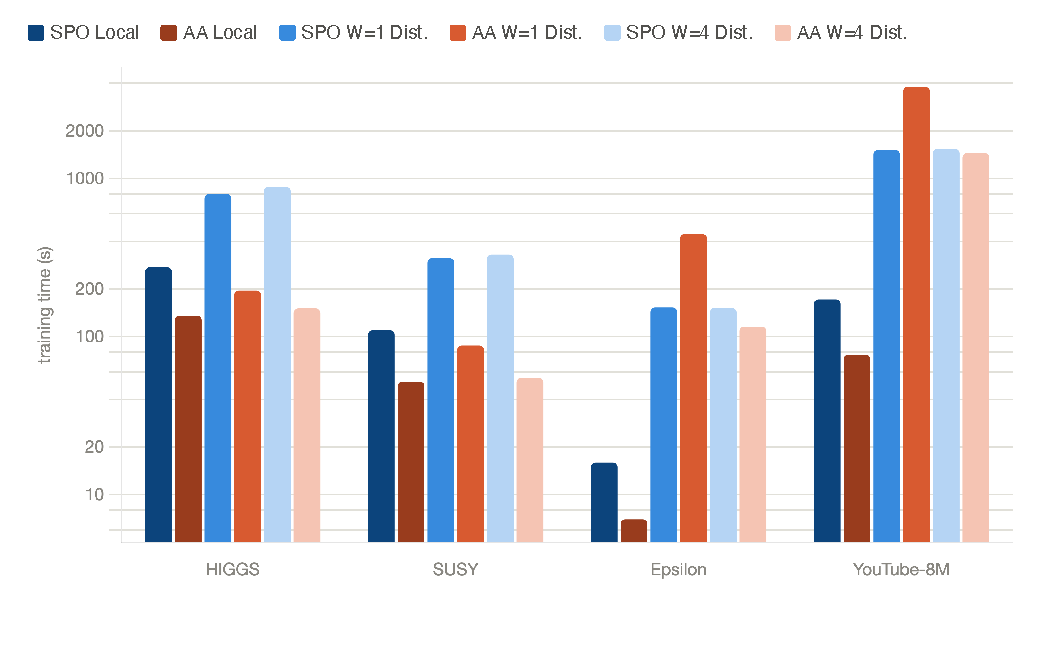
\includegraphics[width=0.75\textwidth]{figures/evaluation/multi_thread_m7i_metal_24x/dist_runtime_bars_chat.pdf}
    \caption{Training time of Dist-GBT (\texttt{MULTI\_THREAD}) vs. Local}
    \label{fig:placeholder}
\end{center}
}]
\clearpage

\subsection{In-node Dist-SPO Parallelism}
\label{sec:in-node-parallelism}

See results at \ref{tab:in-node-dist-vqsort-ablation}, \ref{tab:in-node-dist-vqsort-vertex}

Local SPO only parallelizes in-node when >10 projections. If you see this, ensure $P=F$. Dist SPO-GBT parallel + VQSort implemented 25-Oct-2026

22-Oct-26: \textbf{Added In-node parallelism in SPO-GBT}. single machine gives 2x. Need to update \& rerun above results. Currently also running HIGGS and EPSILON to confirm

\begin{figure*}[t]
\centering
% auto-generated by benchmarks/src/distributed_spo_gbt/make_paper_tables.py -- regenerate, do not hand-edit

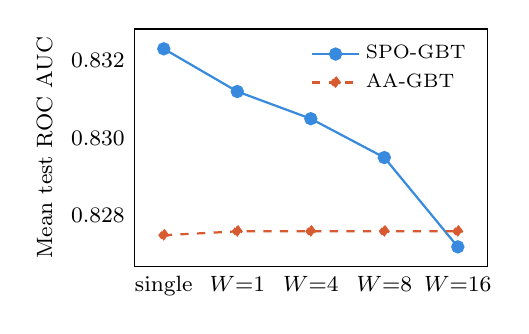
\begin{tikzpicture}
\begin{axis}[width=0.5\textwidth, height=4.6cm, symbolic x coords={Single,1,4,8,16}, xtick=data,
  xticklabels={single,$W{=}1$,$W{=}4$,$W{=}8$,$W{=}16$}, ylabel={Mean test ROC AUC},
  yticklabel style={/pgf/number format/fixed, /pgf/number format/precision=3, /pgf/number format/fixed zerofill},
  tick label style={font=\footnotesize}, label style={font=\footnotesize}, tick style={draw=none},
  legend style={font=\scriptsize, at={(0.98,0.98)}, anchor=north east, draw=none}, legend cell align=left]
\addplot[color={rgb,255:red,55;green,138;blue,221}, mark=*, thick] coordinates {(Single,0.8323) (1,0.8312) (4,0.8305) (8,0.8295) (16,0.8272)};
\addlegendentry{SPO-GBT}
\addplot[color={rgb,255:red,216;green,90;blue,48}, mark=diamond*, thick, dashed] coordinates {(Single,0.8275) (1,0.8276) (4,0.8276) (8,0.8276) (16,0.8276)};
\addlegendentry{AA-GBT}
\end{axis}
\end{tikzpicture}

\caption{Mean test ROC AUC over the datasets of Table~\ref{tab:dist-accuracy}.}
\Description{Line chart of mean AUC versus number of workers for SPO-GBT and AA-GBT.}
\label{fig:dist-accuracy-mean}
\end{figure*}
\clearpage
\begin{table*}[t]
\centering
\footnotesize
\setlength{\tabcolsep}{4pt}
\caption{Benefit of VQSort and distributed in-node parallelism. Tree-training time in seconds on Vertex AI \texttt{n2-highmem-16} ($P{=}F$), ablating Highway VQSort and in-worker parallelism. Models are train byte-identical models.}
\label{tab:in-node-dist-vqsort-ablation}
% auto-generated by benchmarks/src/distributed_spo_gbt/make_pf_ablation_tables.py -- regenerate, do not hand-edit

\begin{tabular}{lrrr}
\toprule
Arm & SUSY ($F{=}18$) & HIGGS ($F{=}28$) & Epsilon ($F{=}2000$) \\
\midrule
AA GBT & 55 & 104 & 132 \\
SPO baseline & 316 & 915 & 1673 \\
SPO + VQSort only & 129 (2.5$\times$) & 403 (2.3$\times$) & 487 (3.4$\times$) \\
SPO + chunk jobs only (\texttt{std::sort}) & 64 (4.9$\times$) & 197 (4.6$\times$) & 335 (5.0$\times$) \\
SPO + both (in-node) & 36 (8.8$\times$) & 116 (7.9$\times$) & 133 (12.6$\times$) \\
\midrule
Acc.\ SPO / AA & 0.7892 / 0.7869 & 0.6923 / 0.6879 & 0.7291 / 0.7192 \\
\bottomrule
\end{tabular}

\par\smallskip\raggedright\footnotesize 10 trees
\end{table*}

\begin{table*}[t]
\centering
\footnotesize
\setlength{\tabcolsep}{4pt}
% (10 trees, depth 6, exact splits)
\caption{Fixing limited SPO in-node parallelism. Training time in seconds of SPO-GBT with $T$ threads on a single \texttt{m7i.24x}. SPO in-node sequential evaluates the $P$ projections in $\min(T,\lceil P/10\rceil)$ threads, i.e.\ single-threaded when $P\le 10$. SPO in-node parallel uses $\min(T,P)$. Existing method was due to PR 403 overhead, which is now gone. TODO $P=F$}
% Used $P=\lceil\sqrt{F}\rceil$.
\label{tab:in-node-dist-vqsort-vertex}
% auto-generated by benchmarks/src/distributed_spo_gbt/make_in_node_tables.py -- regenerate, do not hand-edit
% data: benchmarks/results/runtime/distributed_spo_gbt/in_node_parallelism_2026-10-22/ (run 2026-10-22, m7i.metal-24xl);
% sequential = rebased-main 23053344, parallel = in-node-parallelism-SPOGBT cee3b4c8.

\begin{tabular}{llrrrrrr}
\toprule
Dataset & Arm & \multicolumn{6}{c}{Threads $T$} \\
 & & 1 & 4 & 8 & 16 & 24 & 48 \\
\midrule
HIGGS ($P{=}6$) & SPO in-node sequential & 56.6 & 55.9 & 56.0 & 56.1 & 56.1 & 56.6 \\
 & SPO in-node parallel & 55.8 & 33.4 & 28.1 & 28.8 & 28.2 & 28.9 \\
 & speedup & 1.01$\times$ & 1.67$\times$ & 2.00$\times$ & 1.95$\times$ & 1.99$\times$ & 1.96$\times$ \\
\midrule
SUSY ($P{=}5$) & SPO in-node sequential & 22.3 & \multicolumn{1}{c}{---} & 22.2 & \multicolumn{1}{c}{---} & \multicolumn{1}{c}{---} & 22.6 \\
 & SPO in-node parallel & 22.4 & \multicolumn{1}{c}{---} & 11.1 & \multicolumn{1}{c}{---} & \multicolumn{1}{c}{---} & 11.5 \\
 & speedup & 0.99$\times$ & \multicolumn{1}{c}{---} & 2.00$\times$ & \multicolumn{1}{c}{---} & \multicolumn{1}{c}{---} & 1.97$\times$ \\
\midrule
Epsilon ($P{=}45$) & SPO in-node sequential & 11.8 & 3.80 & 3.12 & 3.20 & 3.38 & 3.26 \\
 & SPO in-node parallel & 12.0 & 3.74 & 2.35 & 1.69 & 1.51 & 1.46 \\
 & speedup & 0.99$\times$ & 1.01$\times$ & 1.32$\times$ & 1.90$\times$ & 2.24$\times$ & 2.24$\times$ \\
\midrule
YouTube-8M ($P{=}34$) & SPO in-node sequential & 100.2 & 33.8 & 33.8 & 34.1 & 34.4 & 34.2 \\
 & SPO in-node parallel & 100.9 & 33.7 & 23.2 & 17.8 & 16.0 & 14.4 \\
 & speedup & 0.99$\times$ & 1.00$\times$ & 1.46$\times$ & 1.91$\times$ & 2.15$\times$ & 2.38$\times$ \\
\bottomrule
\end{tabular}

\end{table*}

\subsection{Call Stack}

\noindent\begin{minipage}{\columnwidth}
\begin{lstlisting}
distributed_gbt.cc::TrainWithStatusImpl()
  ...
  MultiThreadManager()  // MULTI_THREAD, not GRPC
  worker.cc::RunRequest() & RunRequestImpl()
    worker.cc::StartTraining()
      worker.cc::FindSplits()
        training.cc::FindBestSplitsWithThreadPool()
\end{lstlisting}
\end{minipage}


\subsection{Setup cost}

Training a distributed model includes \emph{setup}: the time from job start until the manager logs \texttt{Start tree training} (noted based on whether included). Setup covers reading the CSV from Cloud Storage, building the distributed dataset cache in the shared directory (one file per column, numerical columns presorted) and waiting until every worker has loaded its column partition. (Table~\ref{tab:setup-cost}).

\begin{table}[H]
\centering\footnotesize\setlength{\tabcolsep}{4pt}
\caption{Setup time in seconds (min--max over all runs).}
\label{tab:setup-cost}
% auto-generated by benchmarks/src/distributed_spo_gbt/make_pf_ablation_tables.py -- regenerate, do not hand-edit

\begin{tabular}{lrrr}
\toprule
Dataset & Rows $\times$ cols & \multicolumn{1}{c}{\texttt{n2-highmem-4}} & \multicolumn{1}{c}{\texttt{n2-highmem-16}} \\
\midrule
SUSY & 4.5M $\times$ 18 & 134--262 & 97--185 \\
HIGGS & 10.5M $\times$ 28 & 272--370 & 231--319 \\
Epsilon & 0.4M $\times$ 2000 & 1086--1181 & 997--1045 \\
YouTube-8M & 3.9M $\times$ 1152 & 1908--2024 & 1801--1987 \\
\bottomrule
\end{tabular}

\end{table}


% In-worker sparse oblique splits for distributed GBT (YDF fork, commit 383529b4).
% Source: learner/distributed_decision_tree/oblique.cc (FindBestObliqueSplitForNode,
% EvaluateObliqueSplits) and learner/distributed_gradient_boosted_trees/worker.cc
% (FindSplits, EvaluateSplits). Real code where short; pseudocode for the glue.
\begin{figure*}[t]
\begin{minipage}[t]{0.52\textwidth}
\begin{lstlisting}
// Worker: best oblique split of one open node, using only the
// numerical columns this worker owns (oblique.cc).
void FindBestObliqueSplitForNode(int node, Span<const Idx> rows,
                                 Span<const int> local_feats,
                                 Split* best) {   // holds the AA split
  const int P = GetNumProjections(dt_config, F_numerical);
  const float density = density_factor / local_feats.size();
 
  const int n = rows.size();
  for (int p = 0; p < P; ++p) {
    Projection proj;
    SampleProjection(local_feats, dt_config, density, &proj, &rng);
    // ApplyProjection: gather owned columns at the node's rows.
    for (int i = 0; i < n; ++i) {
      float value = 0;
      for (const auto& [column, weight] : proj)
        value += column[rows[i]] * weight;
      value_and_row[i] = {value, rows[i]};
    }
    // TODO should be HIGHWAY
    std::sort(value_and_row.begin(), value_and_row.end());
    // Exact scan with the axis-aligned scorer
    initializer.InitFull(&pos); initializer.InitEmpty(&neg);
    for (int i = 0, num_pos = n; i < n; ++i, --num_pos) {
      const auto [value, row] = value_and_row[i];
      if (i > 0 && value != value_and_row[i - 1].first &&
          num_pos >= min_examples && num_pos <= n - min_examples) {
        const double score = Score(initializer, pos, neg);
        if (score > best->score)   // beats AA and earlier projections
          *best = {proj, MidThreshold(value_and_row[i-1].first, value),
                   score, /*label stats of both children*/};
      }
      label_filler.Add(row, &neg); label_filler.Sub(row, &pos);
    }
  }
}
\end{lstlisting}
\end{minipage}\hfill
\begin{minipage}[t]{0.46\textwidth}
\begin{lstlisting}
// Worker.cc: FindSplits()
for (node : open_nodes) {
  // Manager's candidate features for this node; all owned here.
  [other, numerical] = PartitionByType(request.features[node]);
  best[node] = AxisAlignedSplitter(other, node);   // stock YDF
}

for (node : open_nodes)
    // one thread-pool job per node
  FindBestObliqueSplitForNode(node, rows_of(node),
                              numerical[node], &best[node]);
reply.splits = best;          // manager keeps the max over workers

// Worker: EvaluateSplits (oblique.cc). The proposer owns every
// attribute of its projection, so it alone writes its bitmap;
// the bitmap is shared exactly as for axis-aligned splits.
for (ex : examples) {
  node = example_to_node[ex];
  if (!winner[node].is_oblique()) continue;
  if (!owns(winner[node])) continue;   // proposed elsewhere
  float value = 0;
  for (const auto& [column, weight] : winner[node].terms)
    value += column[ex] * weight;
  bitmap[node].Write(value >= winner[node].threshold);
}
// Feature ownership is frozen: dynamic load balancing is off.
\end{lstlisting}
\end{minipage}
\caption{In-worker sparse oblique split search in the distributed GBT worker. Left: the per-node search over the worker's own numerical columns (projection sampling, projection evaluation, exact scan). Right: the manager and worker glue around it, and the bitmap evaluation by the proposing worker.}
\label{lst:in_worker_oblique}
\end{figure*}


\section{Work log - Weekly TODOs}

\TODO{Ariel TODOs by Nov-10}

\begin{enumerate}
    \item Column Partitioning: Use a 1\% subset of rows, decide feature importance on this, then use this to distribute for the 100\% dataset
\end{enumerate}


\TODO{Ariel TODOs by Oct-26}

Done:
\begin{enumerate}
    \item Implement VQSort and SPO in-node parallelism
    \item Scale results to GRPC , two instances
    \item Pareto of columns picked
\end{enumerate}

\textbf{\textit{Timing}}
\begin{enumerate}
    \item Time to train -> time at barrier -> time to sync bitmap
    \item Skew to reach barrier
\end{enumerate}

At some point we need datasets that dont fit on 1 machine

\textbf{\textit{Measure accuracy cost of parititioning columns: }}

\begin{enumerate}
    \item full data on each worker
    \item partial data on each: random assignment. 1 column on each
    \item Store all Choose(2) permutations
    
    \item Smart partition strategies
    \begin{itemize}
        \item Correlated columns, put them: (together? apart?)
        \item by some column score
        \item Jovo informative columns
        \item Columns that are split at most often. Usually same columns get picked. \textbf{Implement visualization of this} on natural data
        \item method X - vova?
    \end{itemize}
\end{enumerate}


Extend this to: 1) put globally most important columns in all nodes.
2) v2: put columns that are together most important (i.e. projections) are most important - put them together



\textbf{\textit{Ariel TODOs by Oct-17}}
\begin{todolist}
    \item[\done] Run on actual remove with GRPC
    \item[\done] Disable Turbo boost and SMT in GCP. These settings are not controllable in GCP. We'll need to run multiple experiments
    \item RB good experiment: All data to all workers experiments. Makes SPO very alike AA
    \item run accuracy for multiple seeds
    \item sample features w. replacement per worker. Ensure each column is in at least 1 worker.
    \item  \href{https://github.com/google/yggdrasil-decision-forests/commit/2fe3a7fae5a3e8646401cd98f5c0a2a9d5d81653}{Richard's new} AA + SPO scan.
\end{todolist}





\subsection{Full Implementation Code}

\end{document}
